%!TEX root = ../main.tex
% %

\begin{appendices}

\section{Results by Model}
\subsection{Model 1}

\begin{table}[h!]
\centering
\begin{tabular}{||c c c c c||} 
\hline
Image &  Ground Truth &  Model Count &  Num. Error &    \% Error \\
\hline\hline
37 &            81 &            7 &          74 &  91.358025 \\
39 &            58 &            6 &          52 &  89.655172 \\
41 &            86 &            7 &          79 &  91.860465 \\
44 &           102 &           10 &          92 &  90.196078 \\
\hline
\end{tabular}
\caption{Counts \& errors for Model 1}
\label{count_1}
\end{table}

\begin{figure}[h!]
\subfloat{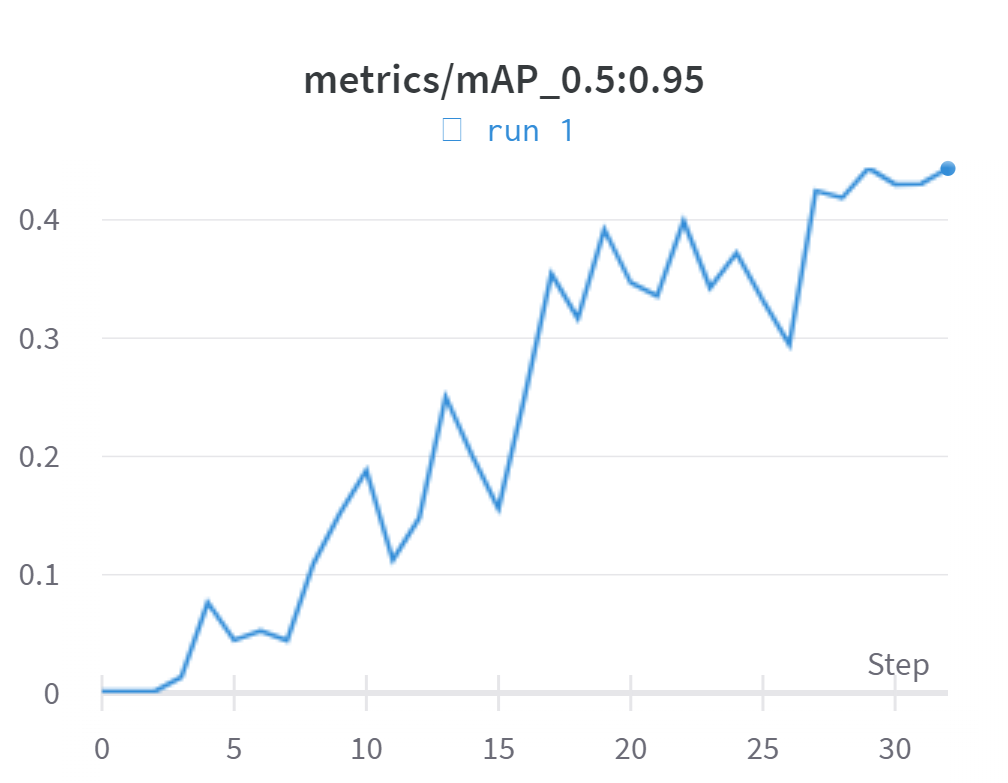
\includegraphics[width=3in]{images/05Testing/run01/Section-2-Panel-0-l24a15v4n}}
\subfloat{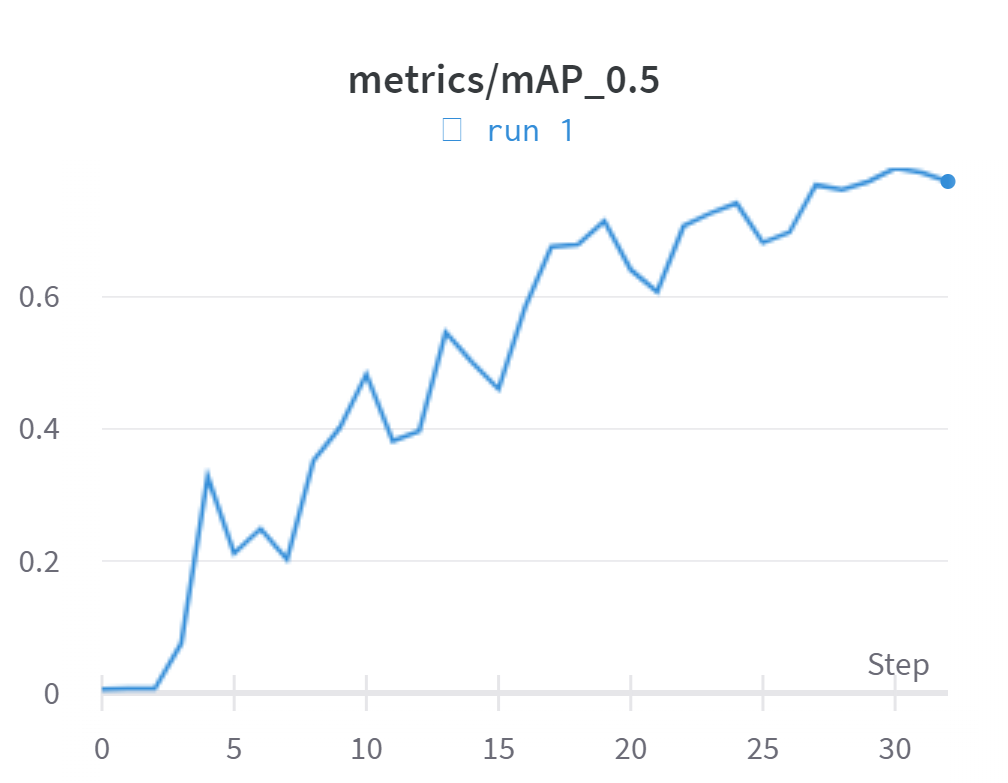
\includegraphics[width=3in]{images/05Testing/run01/Section-2-Panel-1-xq6pmkk16}}\\
\subfloat{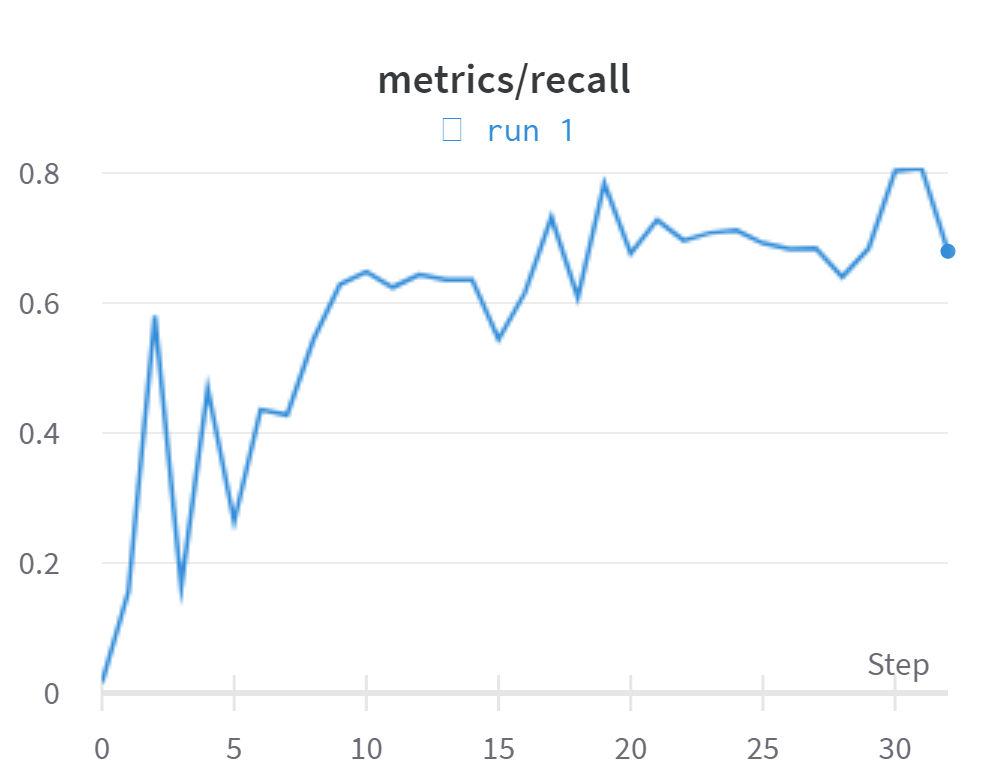
\includegraphics[width=3in]{images/05Testing/run01/Section-2-Panel-2-45rd7tgay}}
\subfloat{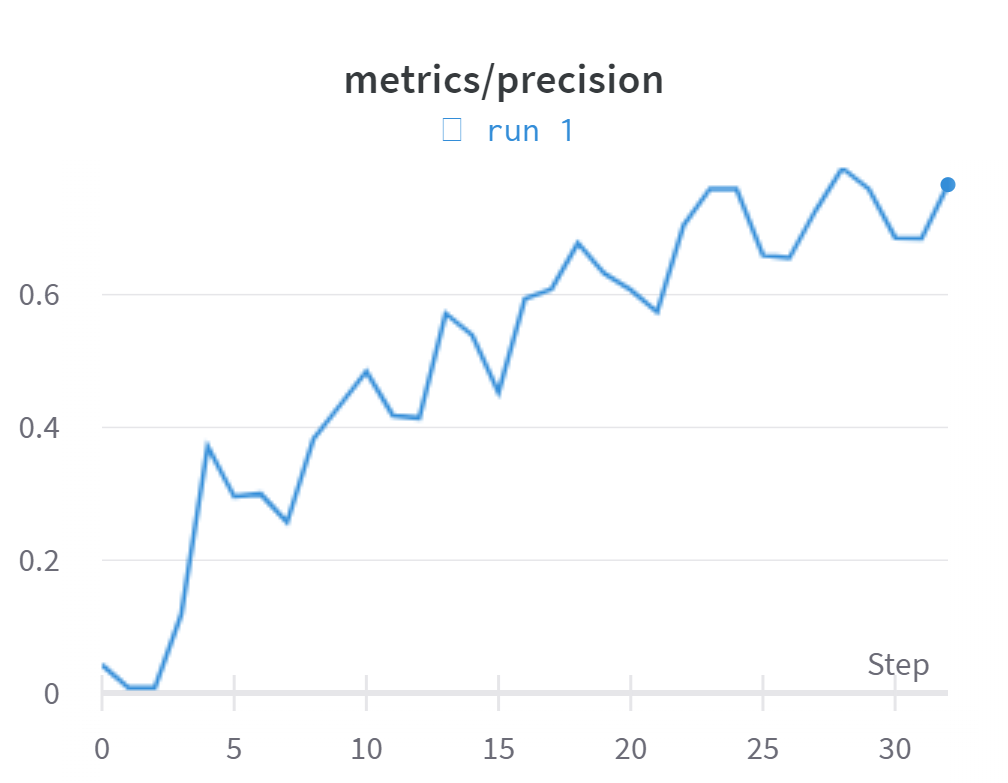
\includegraphics[width=3in]{images/05Testing/run01/Section-2-Panel-3-jsgjesr4f}}\\
\subfloat{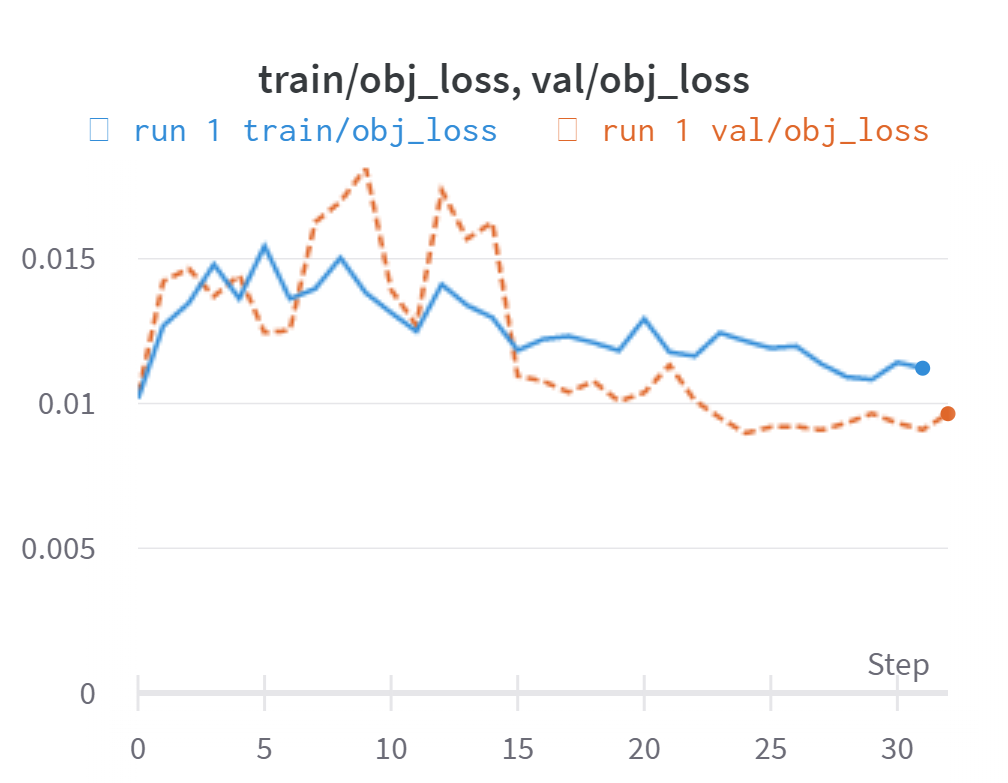
\includegraphics[width=3in]{images/05Testing/run01/Section-2-Panel-4-jgehu72sd}}
\subfloat{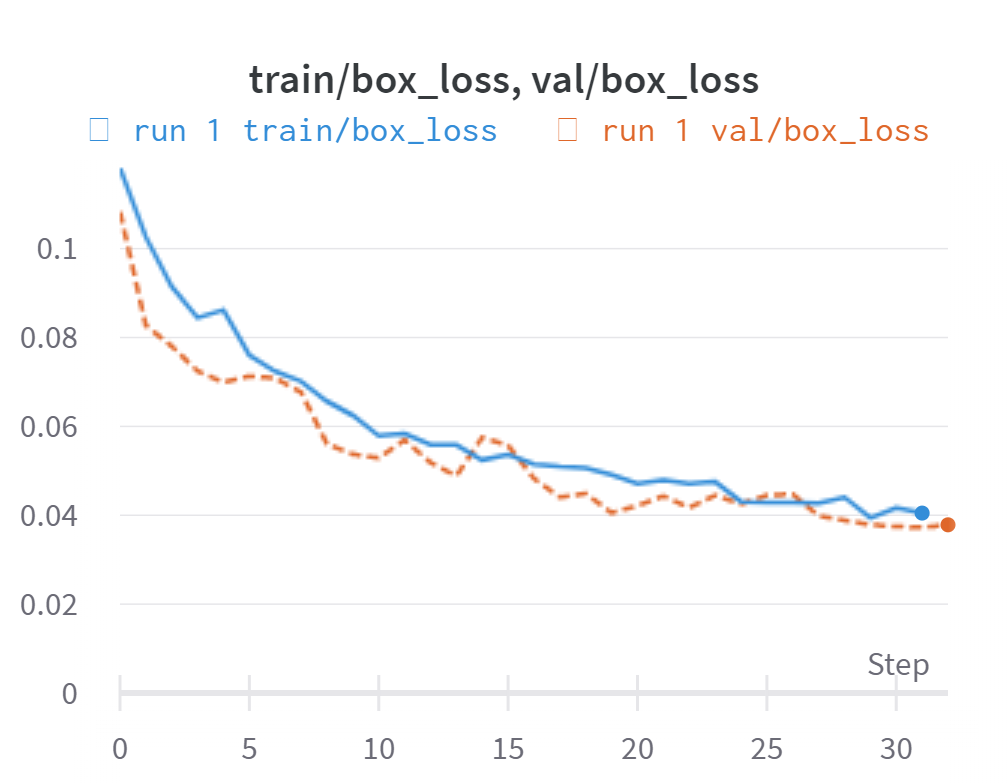
\includegraphics[width=3in]{images/05Testing/run01/Section-2-Panel-5-m94dwffr9}}
\caption{Metrics for Model 1}
\end{figure}

\begin{figure}[h!]
\subfloat{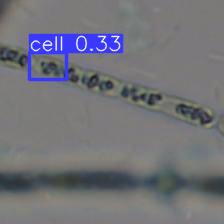
\includegraphics[width=3in]{images/05Testing/run01/easy}}
\subfloat{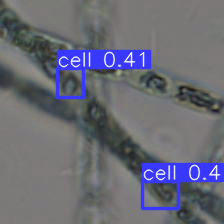
\includegraphics[width=3in]{images/05Testing/run01/hard}}
\caption{Predictions on 'easy' (left) and 'hard' (right) images from the test set by Model 1}
\end{figure}

\subsection{Model 2}

\begin{figure}[h!]
\subfloat{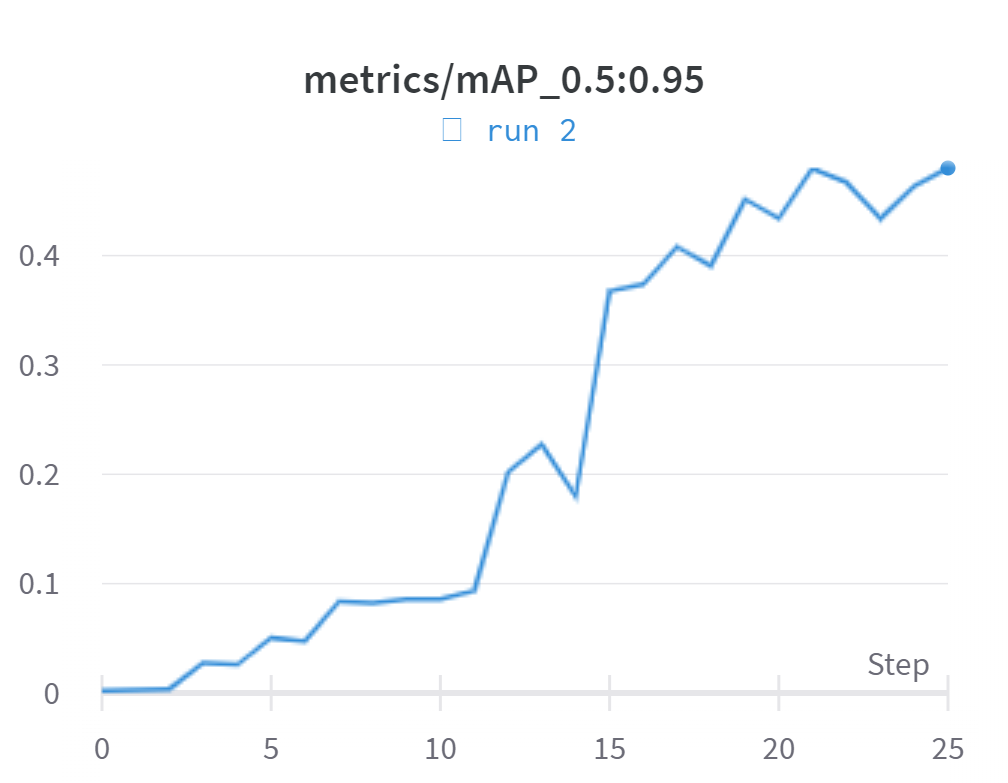
\includegraphics[width=3in]{images/05Testing/run02/Section-2-Panel-0-l24a15v4n}}
\subfloat{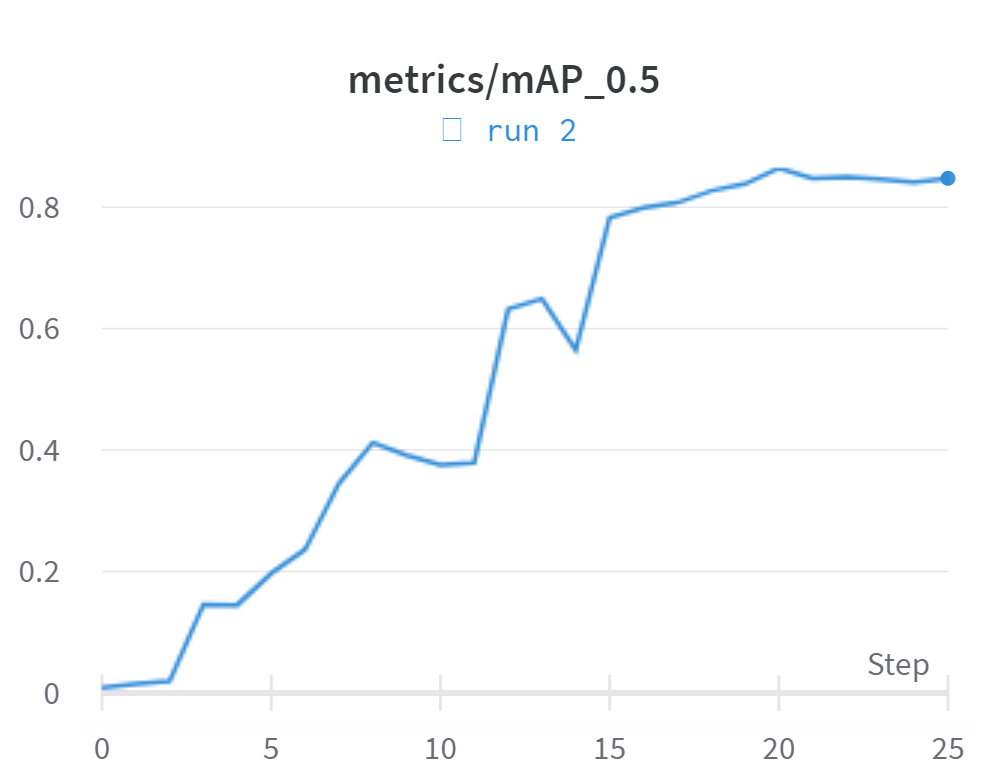
\includegraphics[width=3in]{images/05Testing/run02/Section-2-Panel-1-xq6pmkk16}}\\
\subfloat{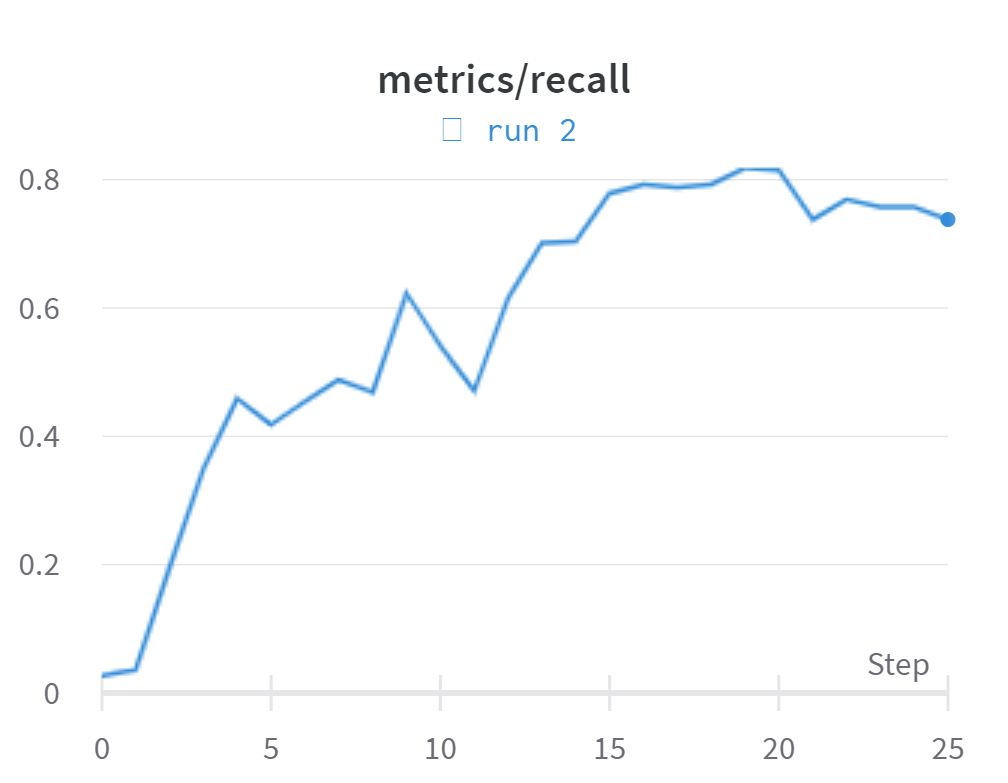
\includegraphics[width=3in]{images/05Testing/run02/Section-2-Panel-2-45rd7tgay}}
\subfloat{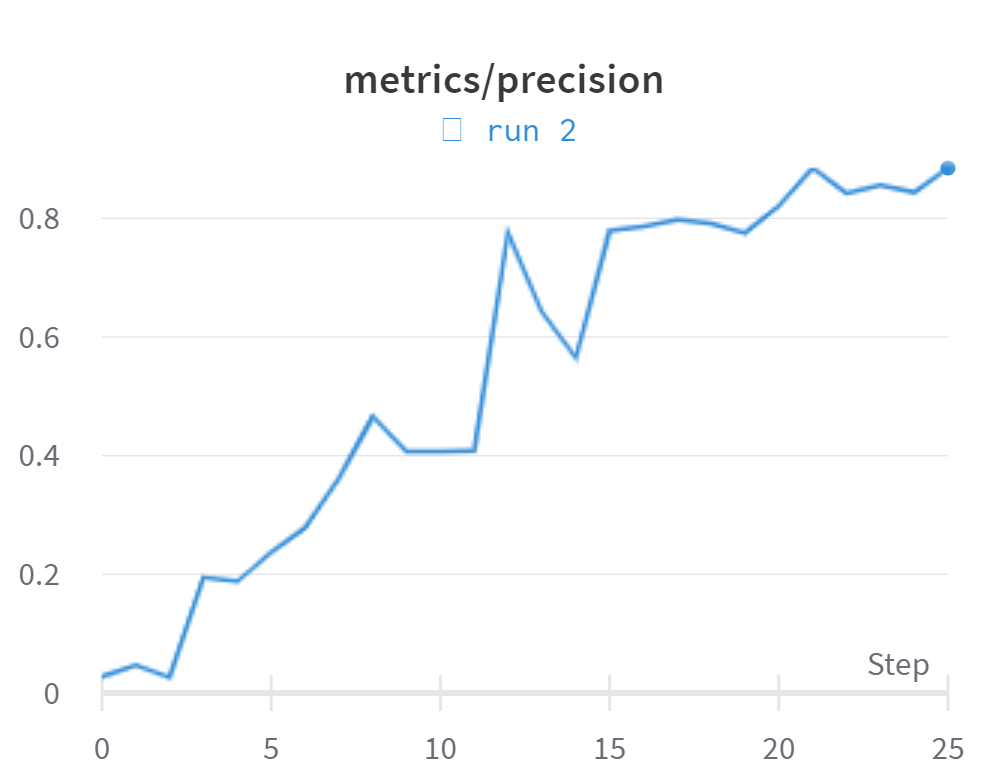
\includegraphics[width=3in]{images/05Testing/run02/Section-2-Panel-3-jsgjesr4f}}\\
\subfloat{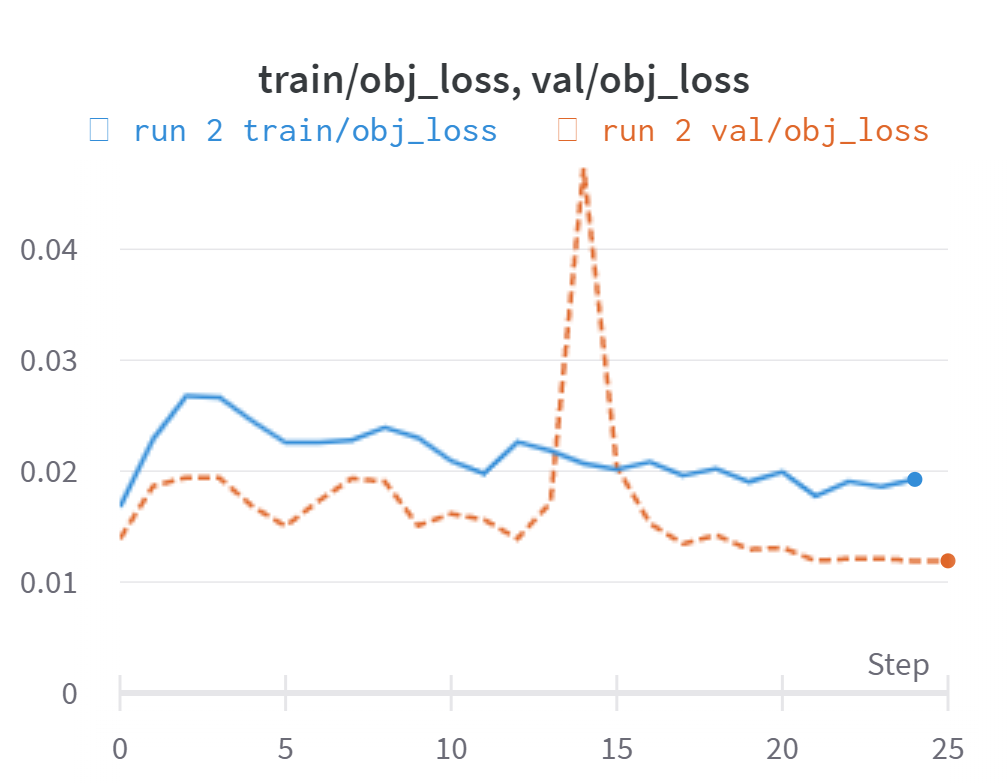
\includegraphics[width=3in]{images/05Testing/run02/Section-2-Panel-4-jgehu72sd}}
\subfloat{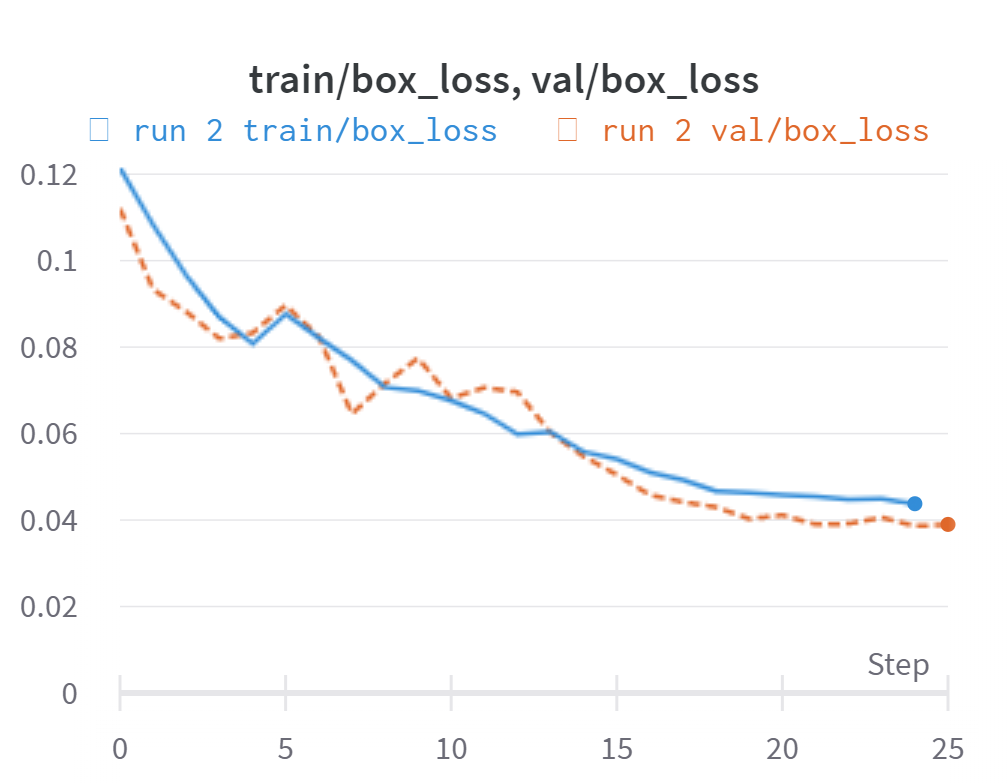
\includegraphics[width=3in]{images/05Testing/run02/Section-2-Panel-5-m94dwffr9}}
\caption{Metrics for Model 2}
\end{figure}

\begin{table}[h!]
\centering
\begin{tabular}{||c c c c c||} 
\hline
Image &  Ground Truth &  Model Count &  Num. Error &    \% Error \\
\hline\hline
37 &            81 &          193 &         112 &  138.271605 \\
39 &            58 &          100 &          42 &   72.413793 \\
41 &            86 &          147 &          61 &   70.930233 \\
44 &           102 &          235 &         133 &  130.392157 \\
\hline
\end{tabular}
\caption{Counts \& errors for Model 2}
\label{count_2}
\end{table}

\subsection{Model 3}

\begin{figure}[h!]
\subfloat{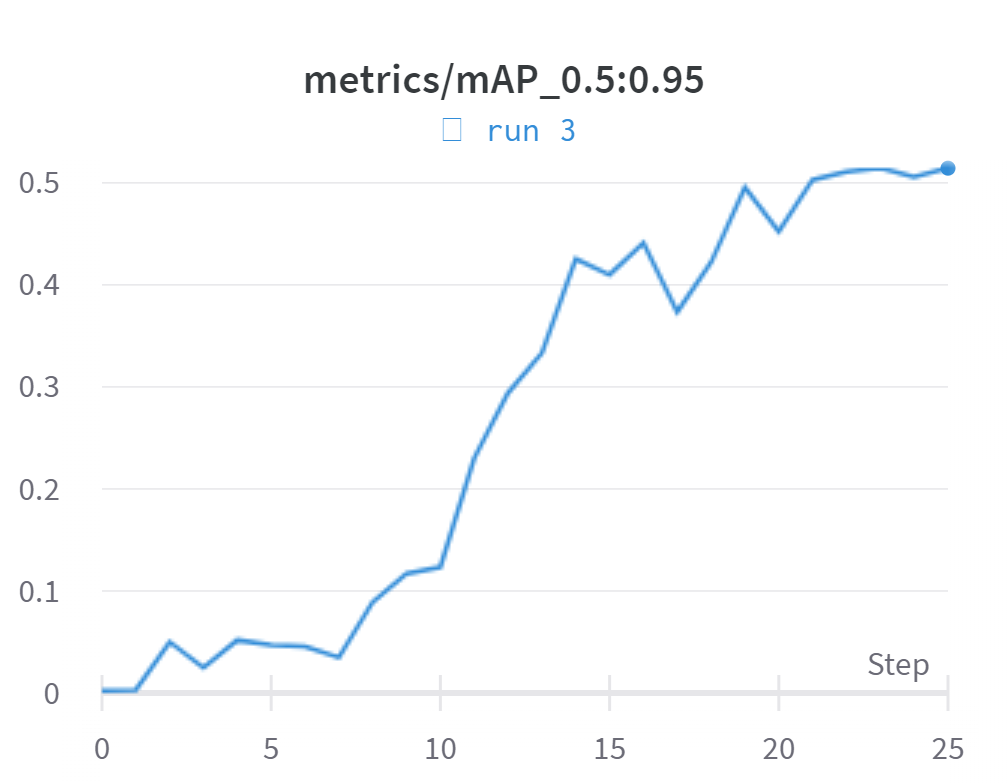
\includegraphics[width=3in]{images/05Testing/run03/Section-2-Panel-0-l24a15v4n}}
\subfloat{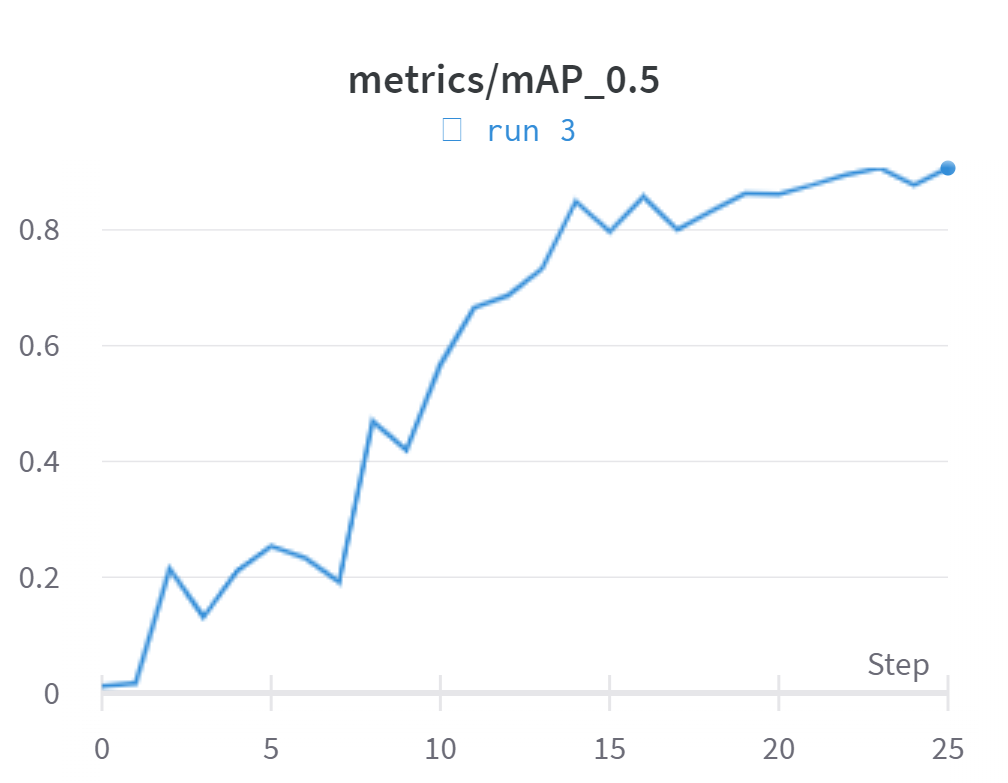
\includegraphics[width=3in]{images/05Testing/run03/Section-2-Panel-1-xq6pmkk16}}\\
\subfloat{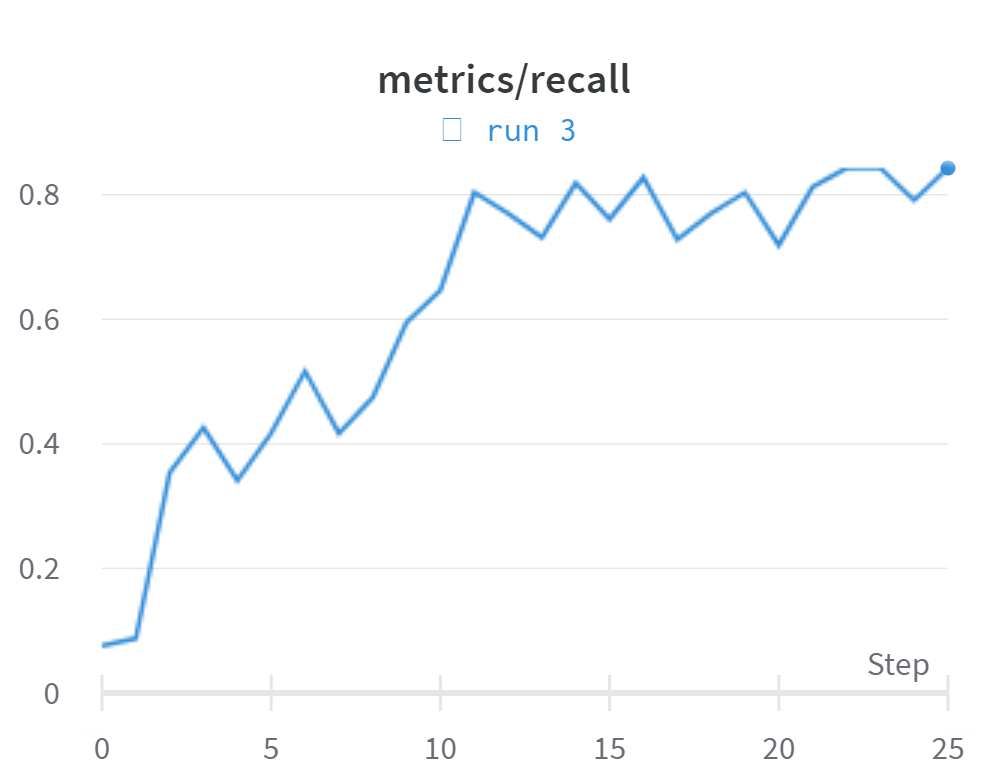
\includegraphics[width=3in]{images/05Testing/run03/Section-2-Panel-2-45rd7tgay}}
\subfloat{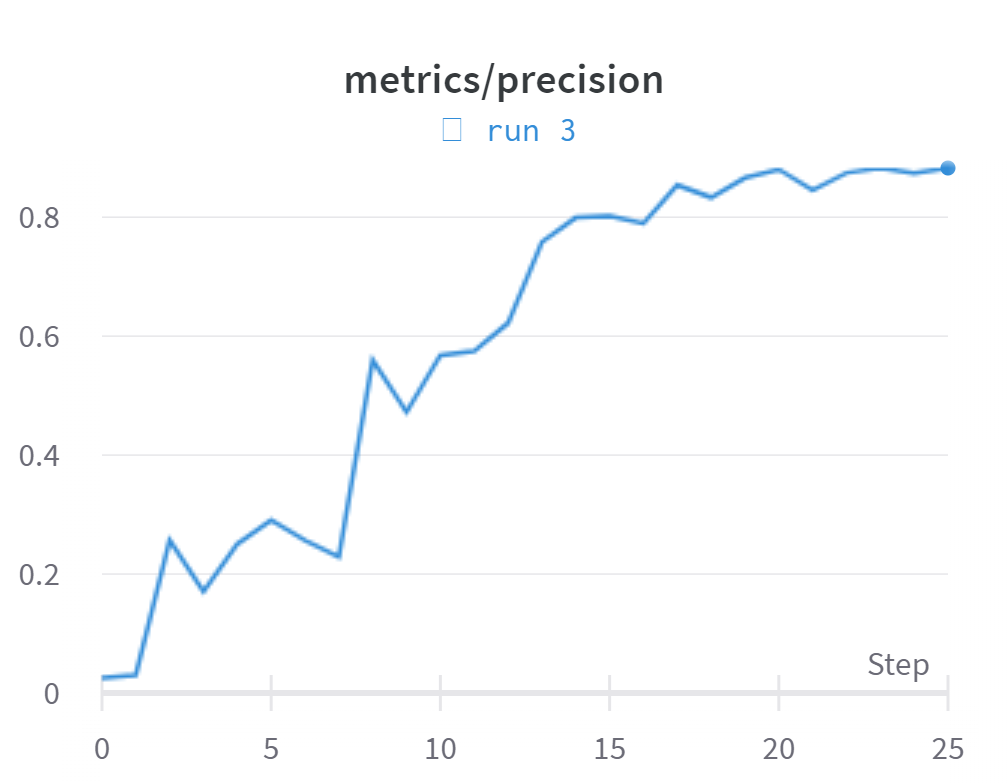
\includegraphics[width=3in]{images/05Testing/run03/Section-2-Panel-3-jsgjesr4f}}\\
\subfloat{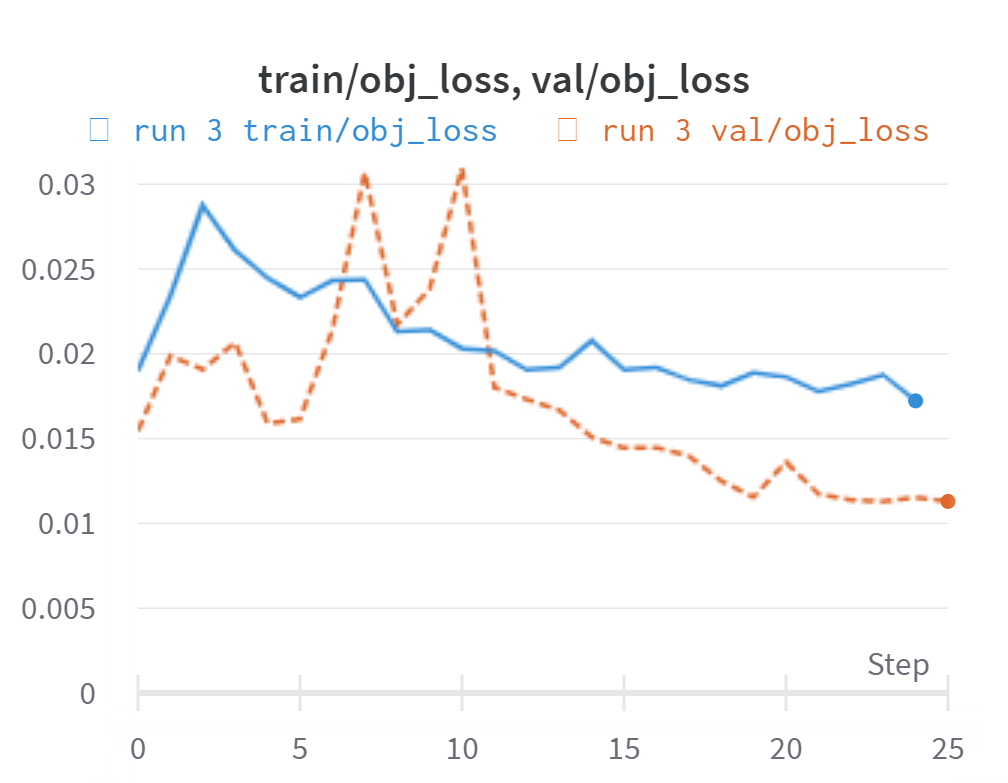
\includegraphics[width=3in]{images/05Testing/run03/Section-2-Panel-4-jgehu72sd}}
\subfloat{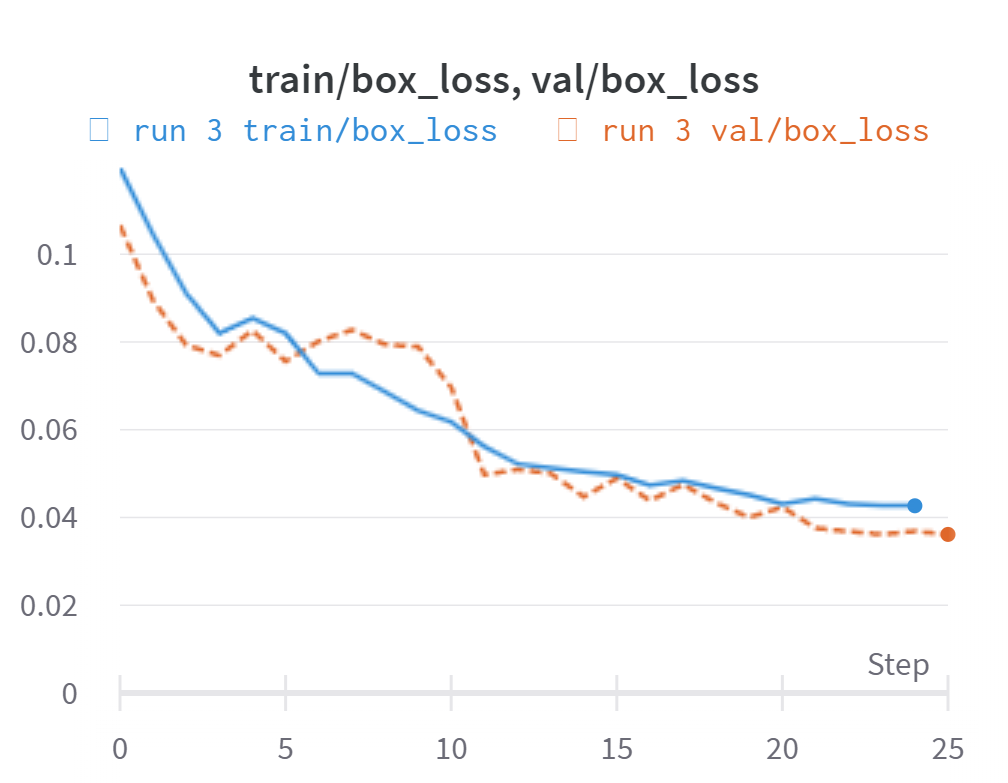
\includegraphics[width=3in]{images/05Testing/run03/Section-2-Panel-5-m94dwffr9}}
\caption{Metrics for Model 3}
\end{figure}

\begin{table}[h!]
\centering
\begin{tabular}{||c c c c c||} 
\hline
Image &  Ground Truth &  Model Count &  Num. Error &    \% Error \\
\hline\hline
37 &            81 &          183 &         102 &  125.925926 \\
39 &            58 &          117 &          59 &  101.724138 \\
41 &            86 &          147 &          61 &   70.930233 \\
44 &           102 &          213 &         111 &  108.823529 \\
\hline
\end{tabular}
\caption{Counts \& errors for Model 3}
\label{count_3}
\end{table}

\subsection{Model 4}

\begin{figure}[h!]
\subfloat{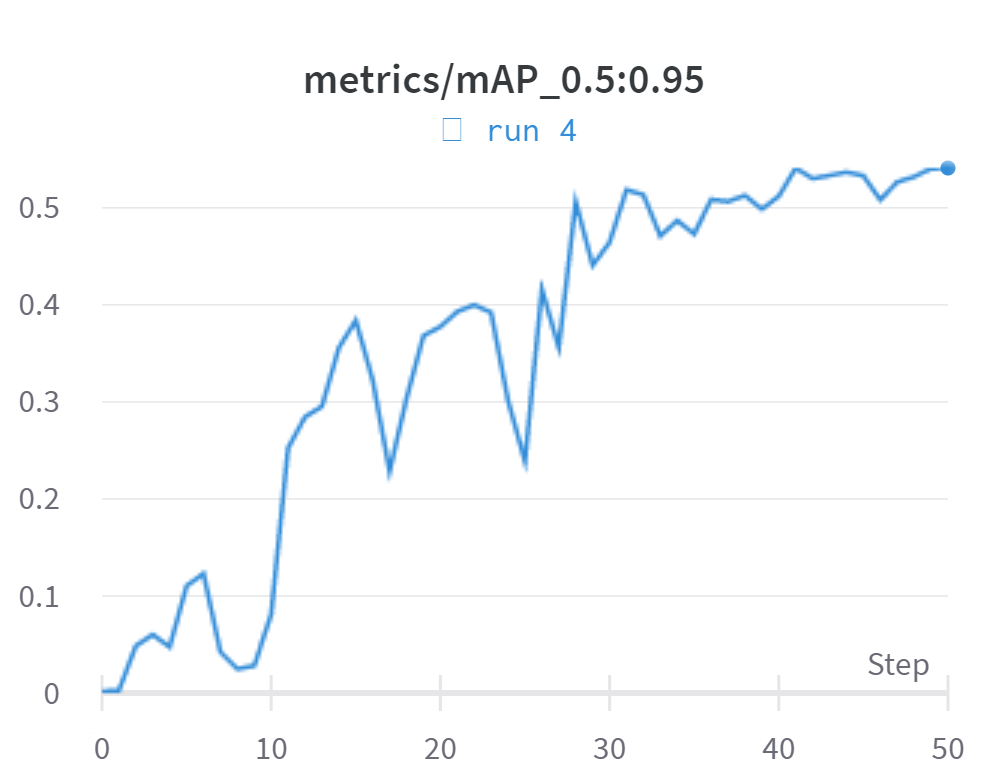
\includegraphics[width=3in]{images/05Testing/run04/Section-2-Panel-0-l24a15v4n}}
\subfloat{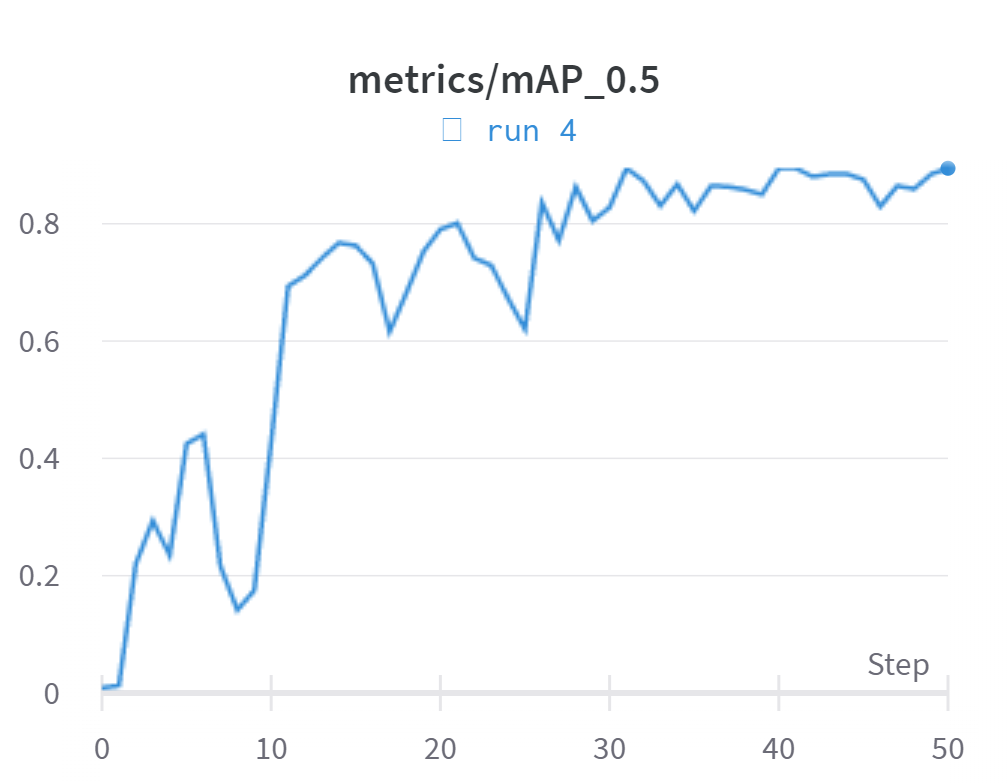
\includegraphics[width=3in]{images/05Testing/run04/Section-2-Panel-1-xq6pmkk16}}\\
\subfloat{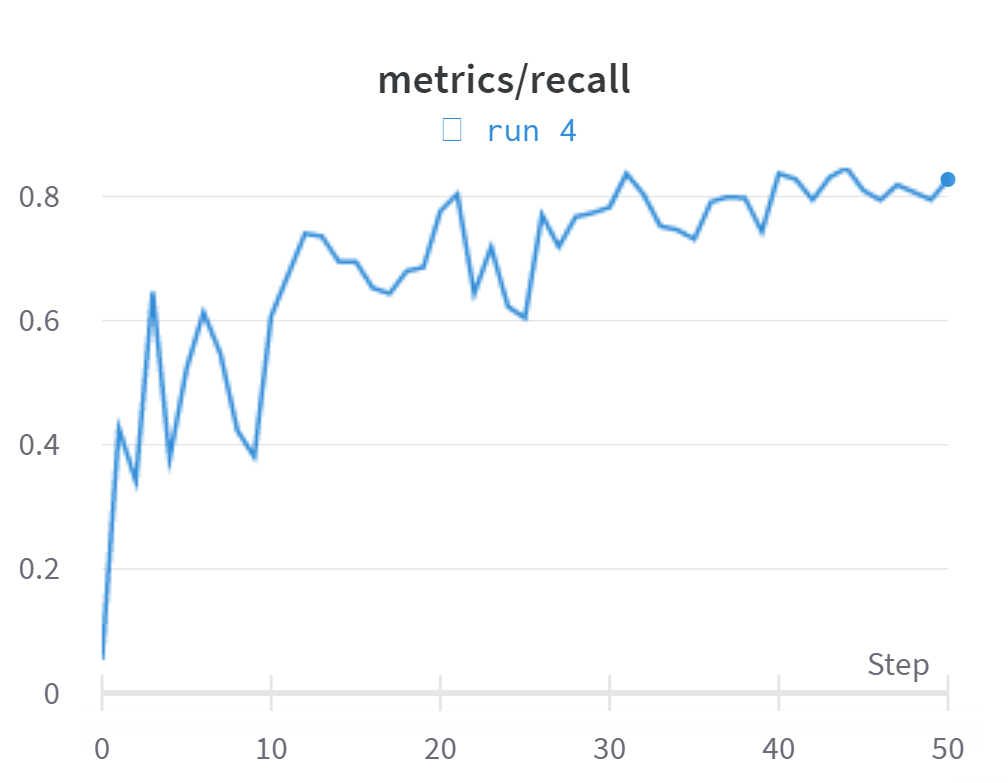
\includegraphics[width=3in]{images/05Testing/run04/Section-2-Panel-2-45rd7tgay}}
\subfloat{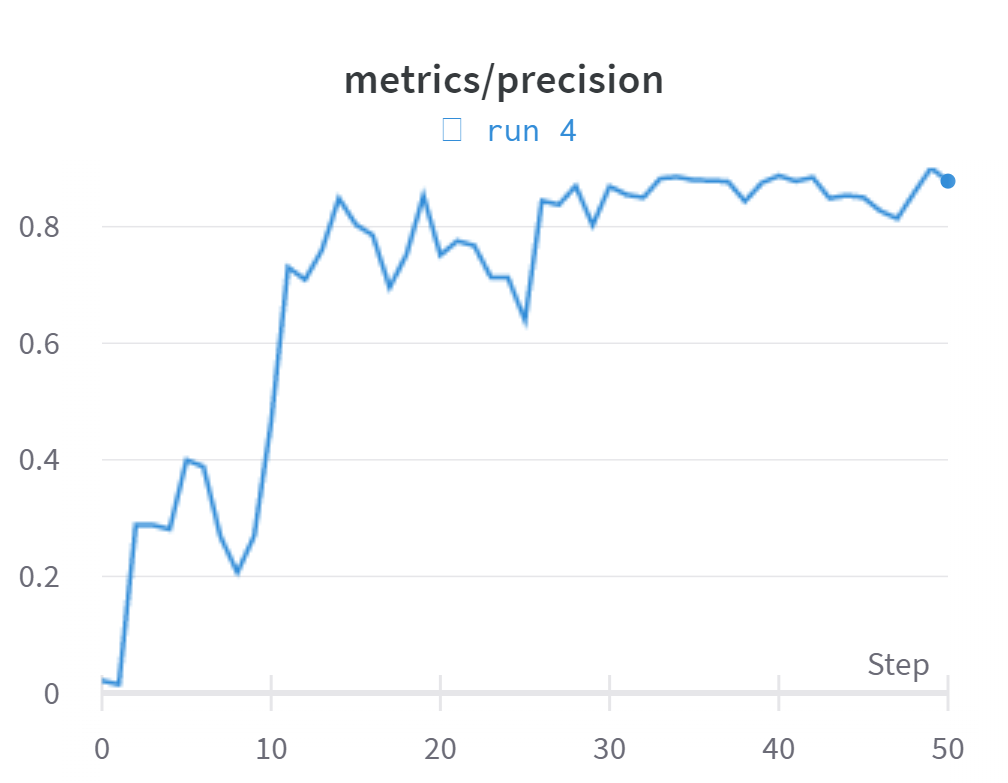
\includegraphics[width=3in]{images/05Testing/run04/Section-2-Panel-3-jsgjesr4f}}\\
\subfloat{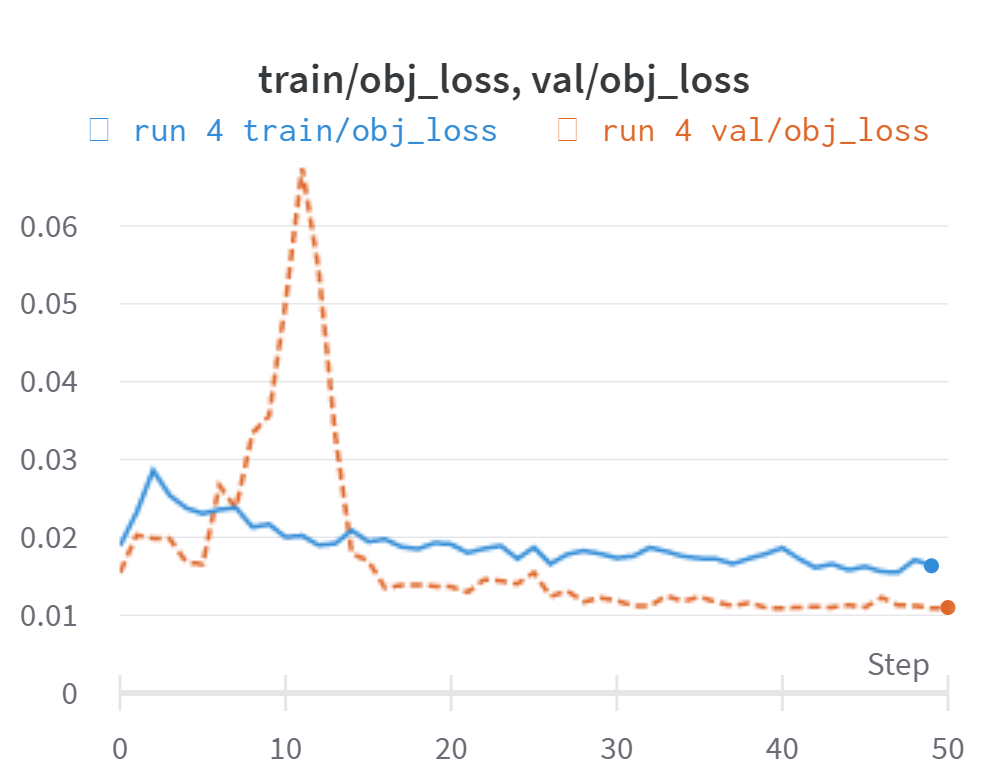
\includegraphics[width=3in]{images/05Testing/run04/Section-2-Panel-4-jgehu72sd}}
\subfloat{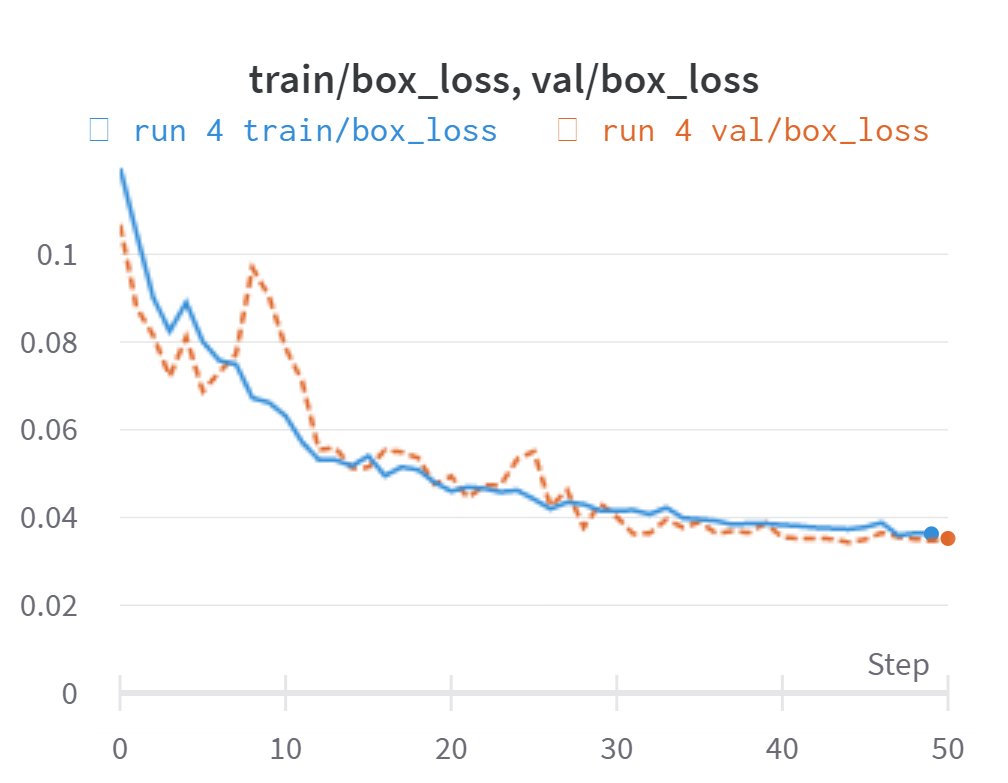
\includegraphics[width=3in]{images/05Testing/run04/Section-2-Panel-5-m94dwffr9}}
\caption{Metrics for Model 4}
\end{figure}

\begin{table}[h!]
\centering
\begin{tabular}{||c c c c c||} 
\hline
Image &  Ground Truth &  Model Count &  Num. Error &    \% Error \\
\hline\hline
37 &            81 &          145 &          64 &  79.012346 \\
39 &            58 &           97 &          39 &  67.241379 \\
41 &            86 &          136 &          50 &  58.139535 \\
44 &           102 &          201 &          99 &  97.058824 \\
\hline
\end{tabular}
\caption{Counts \& errors for Model 4}
\label{count_4}
\end{table}

\subsection{Model 5}

\begin{figure}[h!]
\subfloat{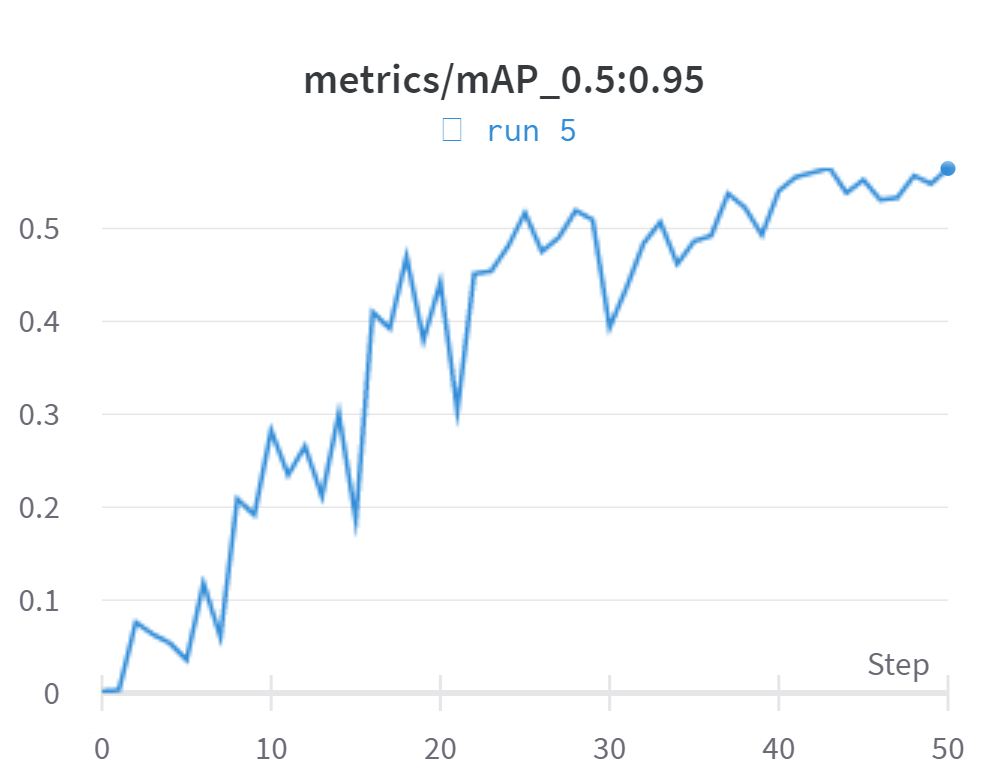
\includegraphics[width=3in]{images/05Testing/run05/Section-2-Panel-0-l24a15v4n}}
\subfloat{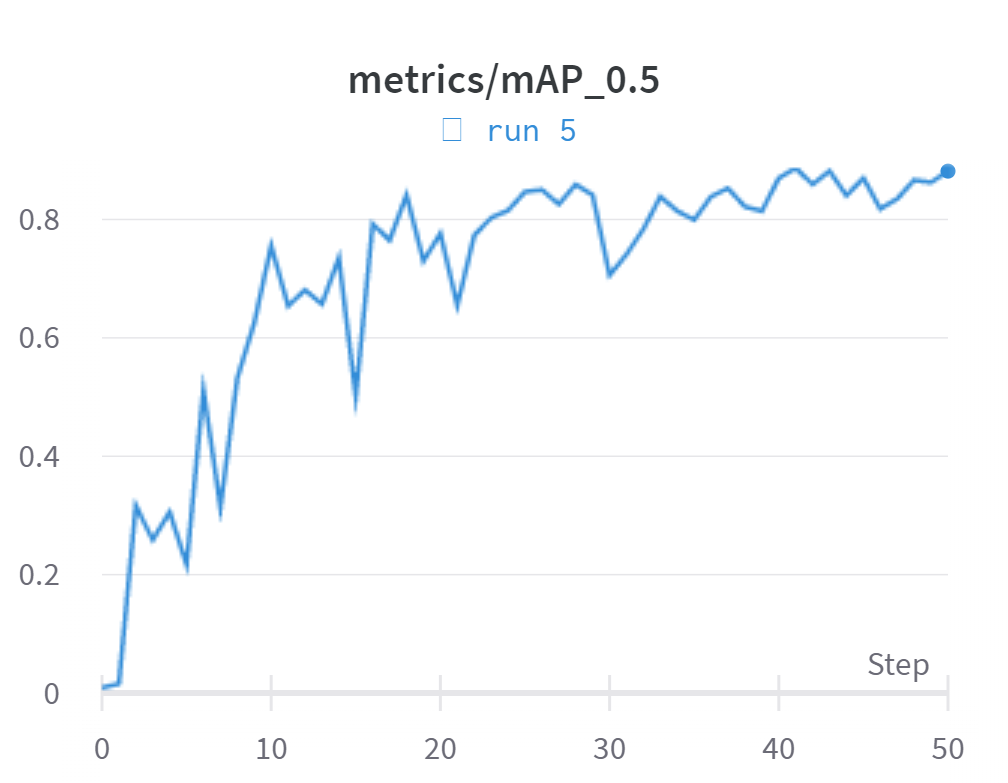
\includegraphics[width=3in]{images/05Testing/run05/Section-2-Panel-1-xq6pmkk16}}\\
\subfloat{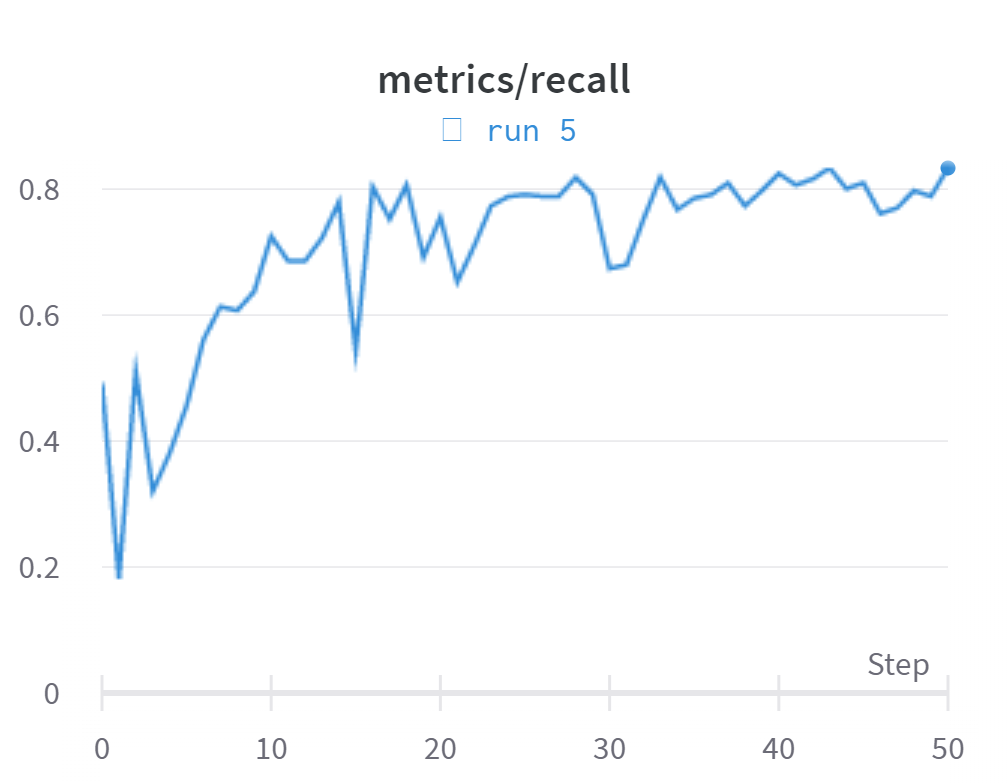
\includegraphics[width=3in]{images/05Testing/run05/Section-2-Panel-2-45rd7tgay}}
\subfloat{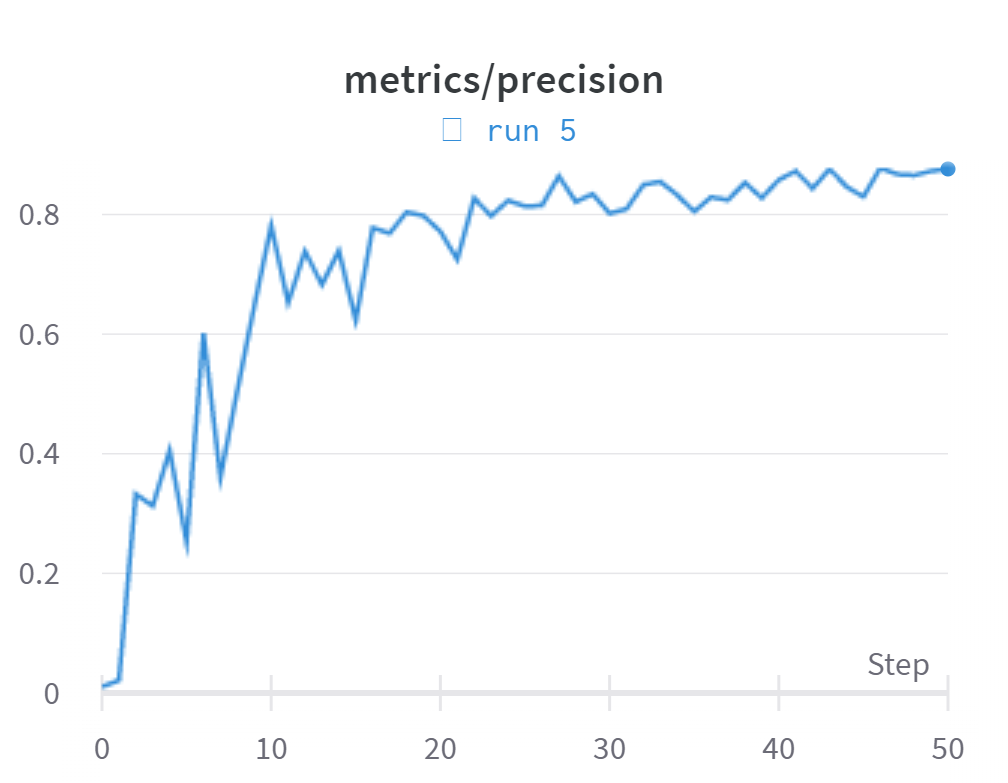
\includegraphics[width=3in]{images/05Testing/run05/Section-2-Panel-3-jsgjesr4f}}\\
\subfloat{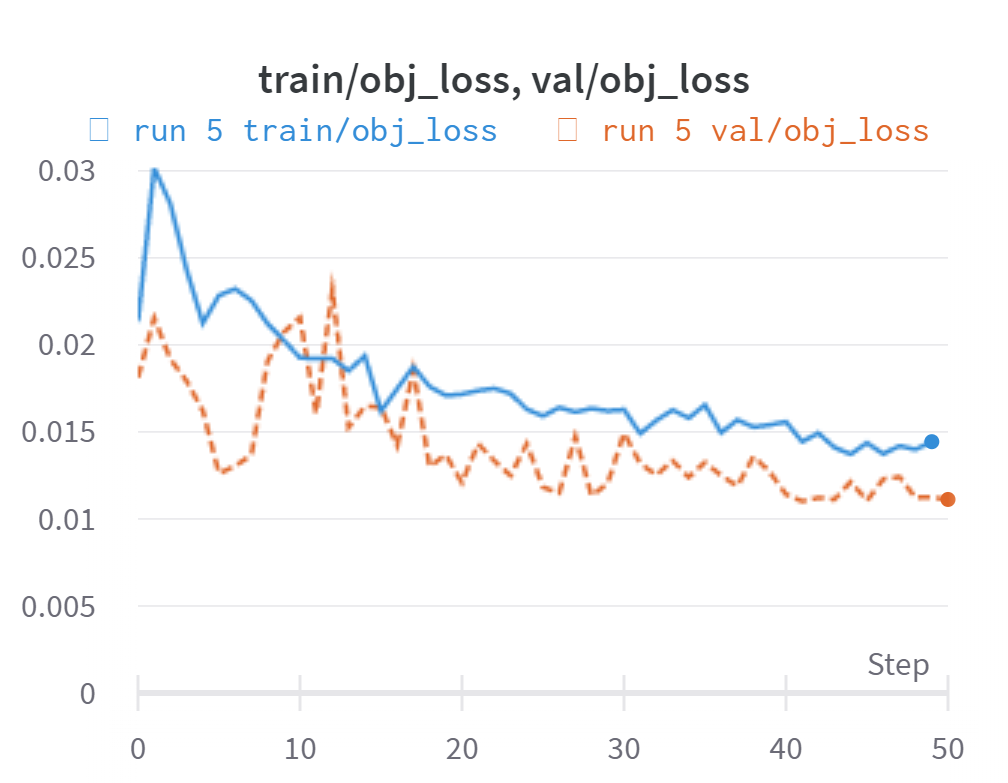
\includegraphics[width=3in]{images/05Testing/run05/Section-2-Panel-4-jgehu72sd}}
\subfloat{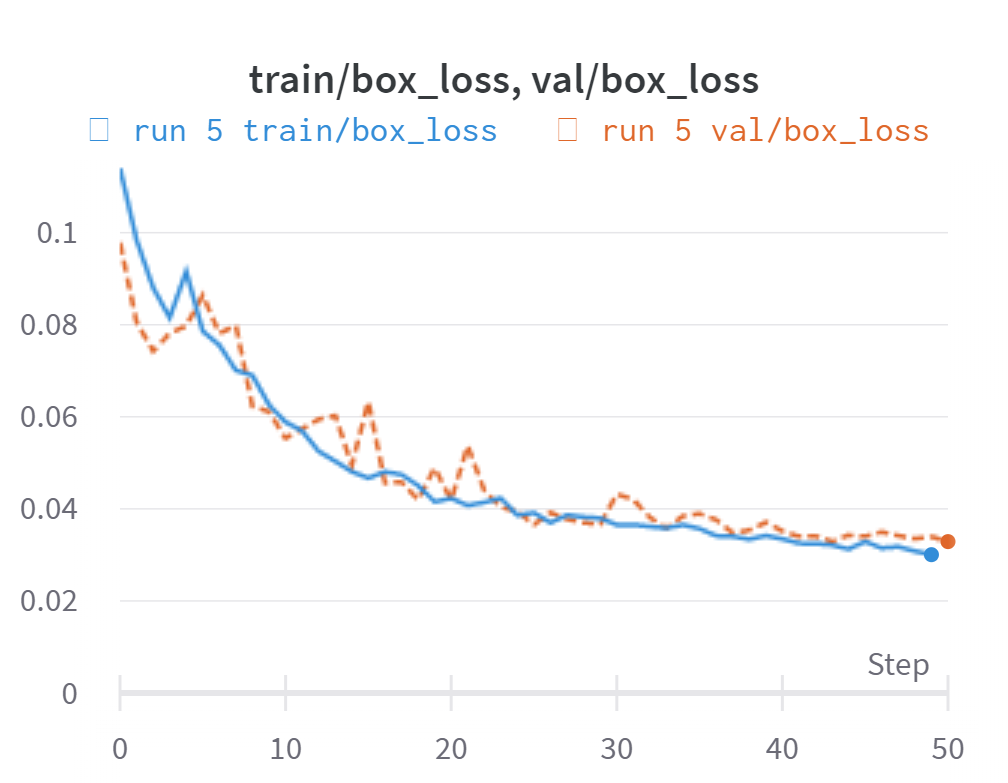
\includegraphics[width=3in]{images/05Testing/run05/Section-2-Panel-5-m94dwffr9}}
\caption{Metrics for Model 5}
\end{figure}

\begin{table}[h!]
\centering
\begin{tabular}{||c c c c c||} 
\hline
Image &  Ground Truth &  Model Count &  Num. Error &    \% Error \\
\hline\hline
37 &            81 &          159 &          78 &  96.296296 \\
39 &            58 &          106 &          48 &  82.758621 \\
41 &            86 &          128 &          42 &  48.837209 \\
44 &           102 &          184 &          82 &  80.392157 \\
\hline
\end{tabular}
\caption{Counts \& errors for Model 5}
\label{count_5}
\end{table}

\subsection{Model 6}

\begin{figure}[h!]
\subfloat{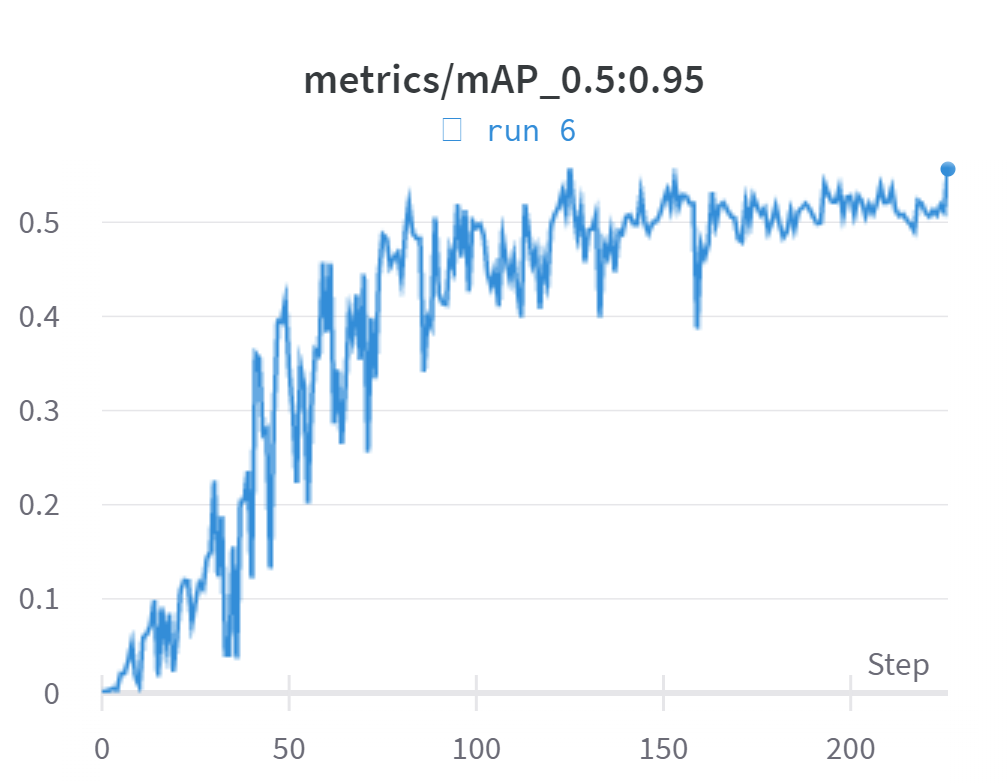
\includegraphics[width=3in]{images/05Testing/run06/Section-2-Panel-0-l24a15v4n}}
\subfloat{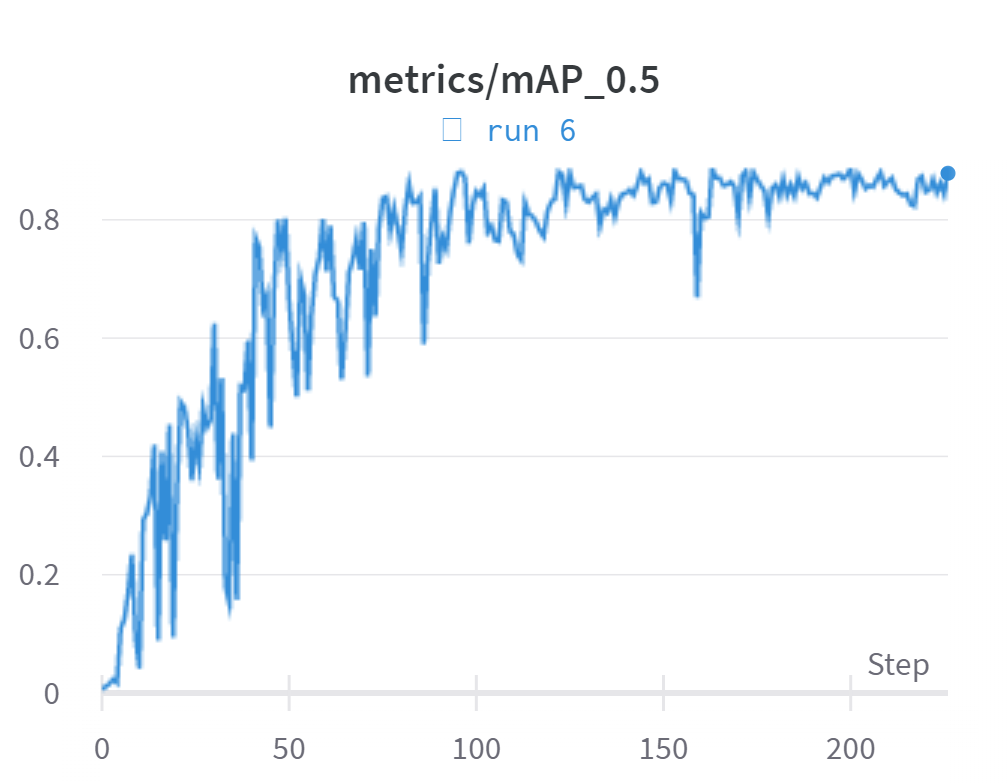
\includegraphics[width=3in]{images/05Testing/run06/Section-2-Panel-1-xq6pmkk16}}\\
\subfloat{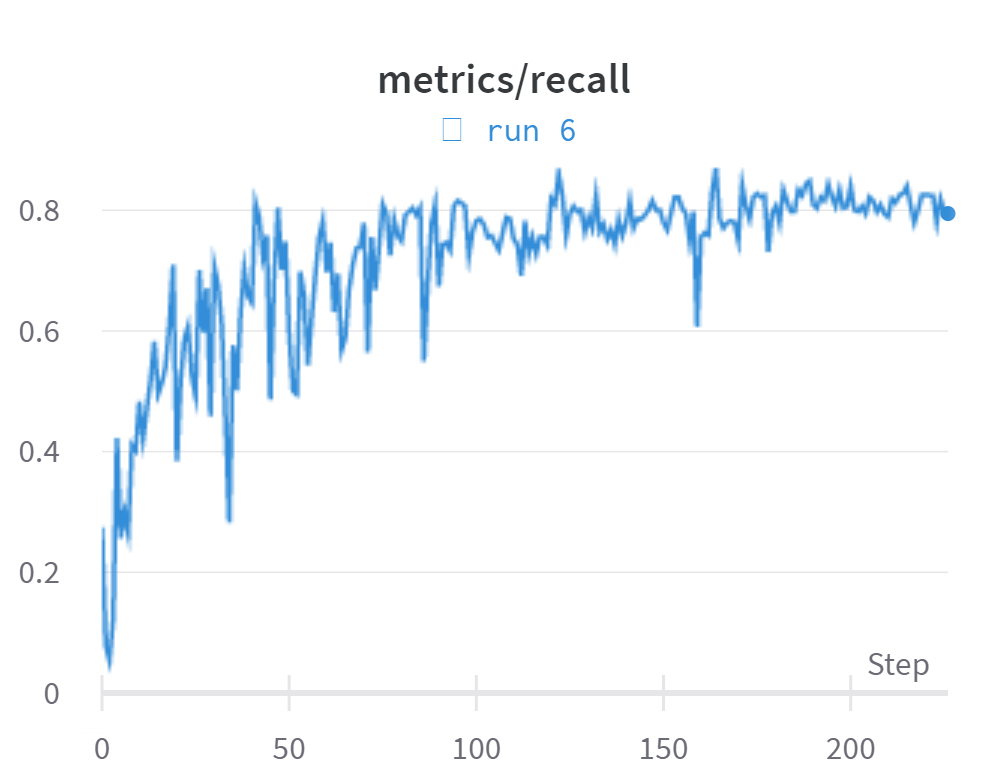
\includegraphics[width=3in]{images/05Testing/run06/Section-2-Panel-2-45rd7tgay}}
\subfloat{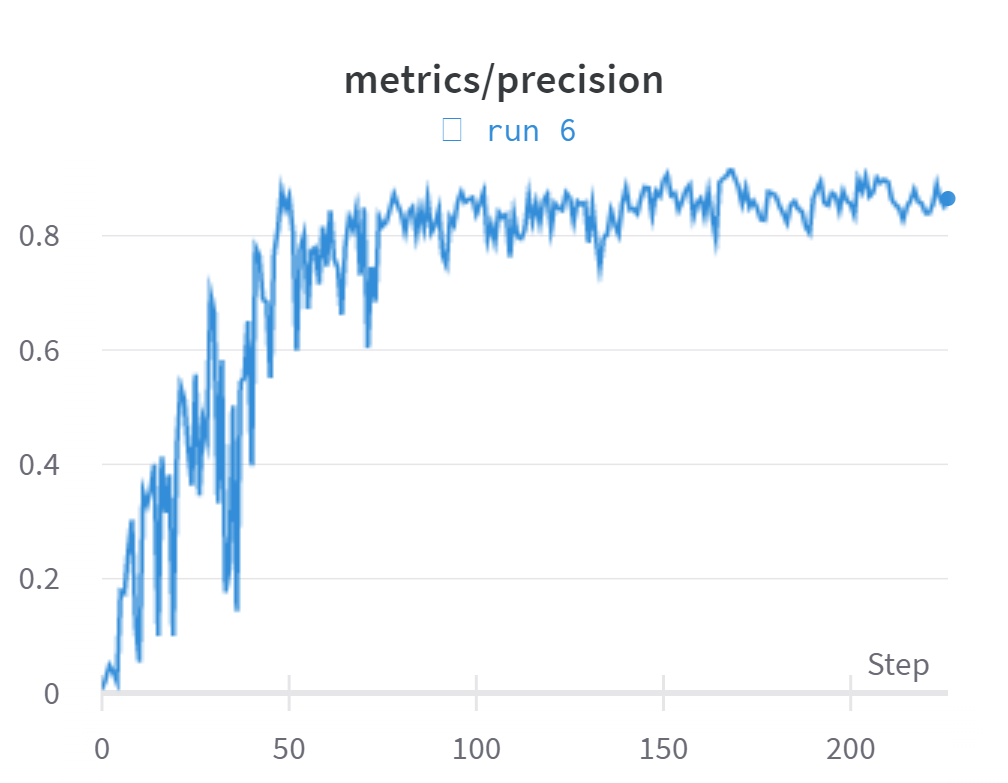
\includegraphics[width=3in]{images/05Testing/run06/Section-2-Panel-3-jsgjesr4f}}\\
\subfloat{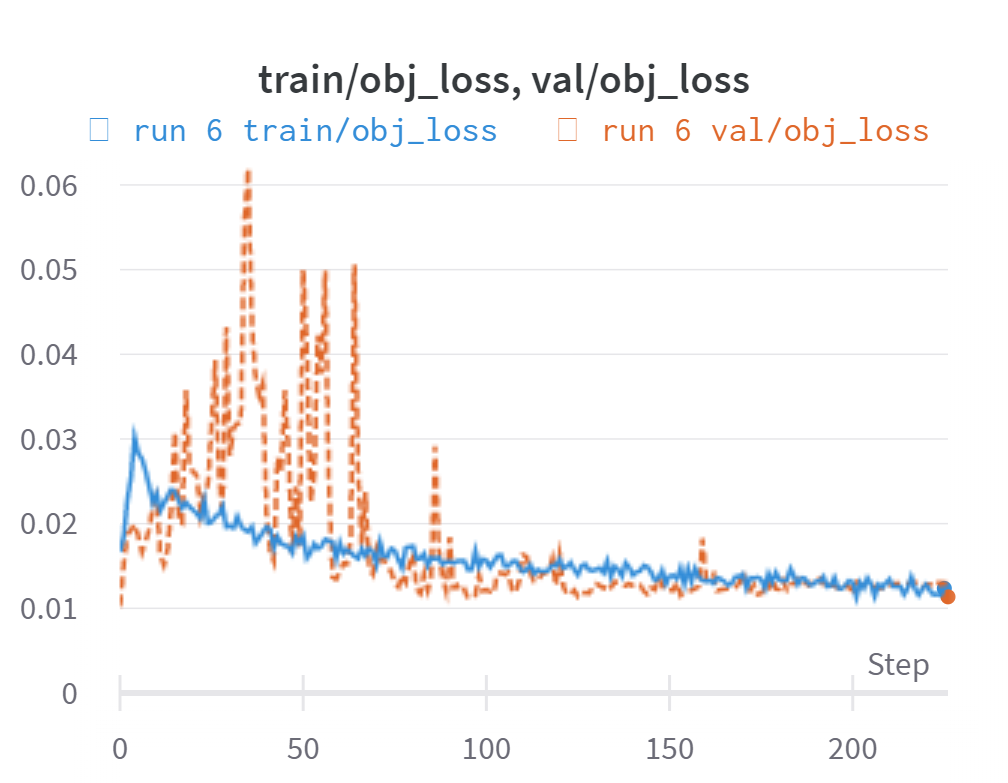
\includegraphics[width=3in]{images/05Testing/run06/Section-2-Panel-4-jgehu72sd}}
\subfloat{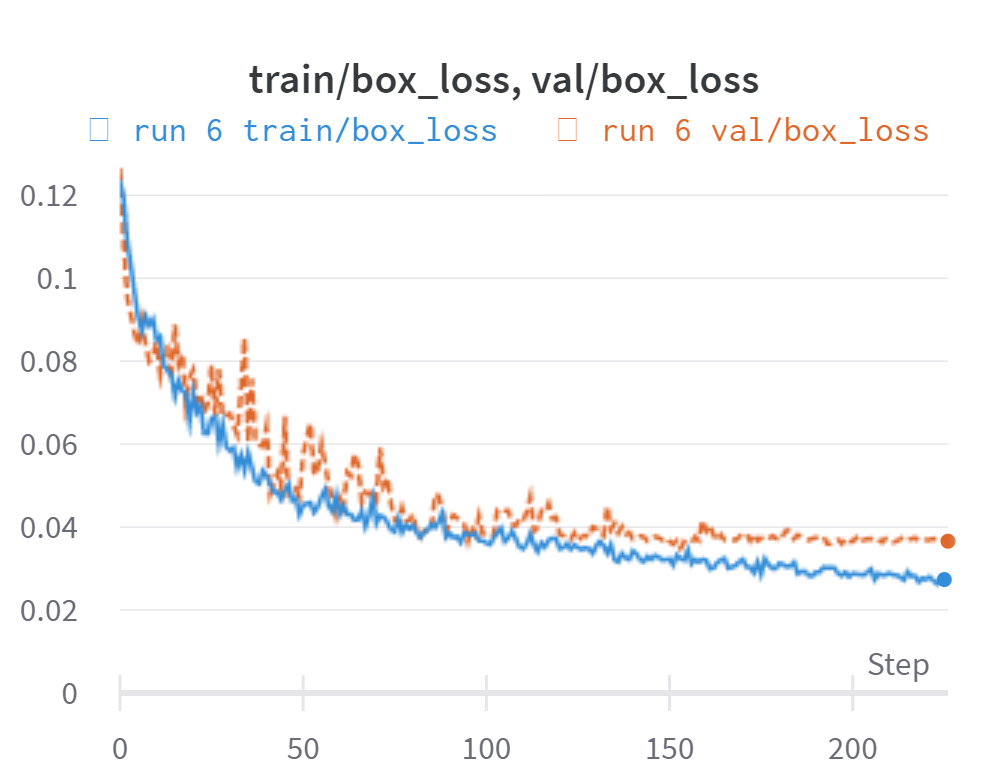
\includegraphics[width=3in]{images/05Testing/run06/Section-2-Panel-5-m94dwffr9}}
\caption{Metrics for Model 6}
\end{figure}

\begin{table}[h!]
\centering
\begin{tabular}{||c c c c c||} 
\hline
Image &  Ground Truth &  Model Count &  Num. Error &    \% Error \\
\hline\hline
37 &            81 &          117 &          36 &  44.444444 \\
39 &            58 &           45 &          13 &  22.413793 \\
41 &            86 &           75 &          11 &  12.790698 \\
44 &           102 &          106 &           4 &   3.921569 \\
\hline
\end{tabular}
\caption{Counts \& errors for Model 6}
\label{count_6}
\end{table}

\subsection{Model 7}

\begin{figure}[h!]
\subfloat{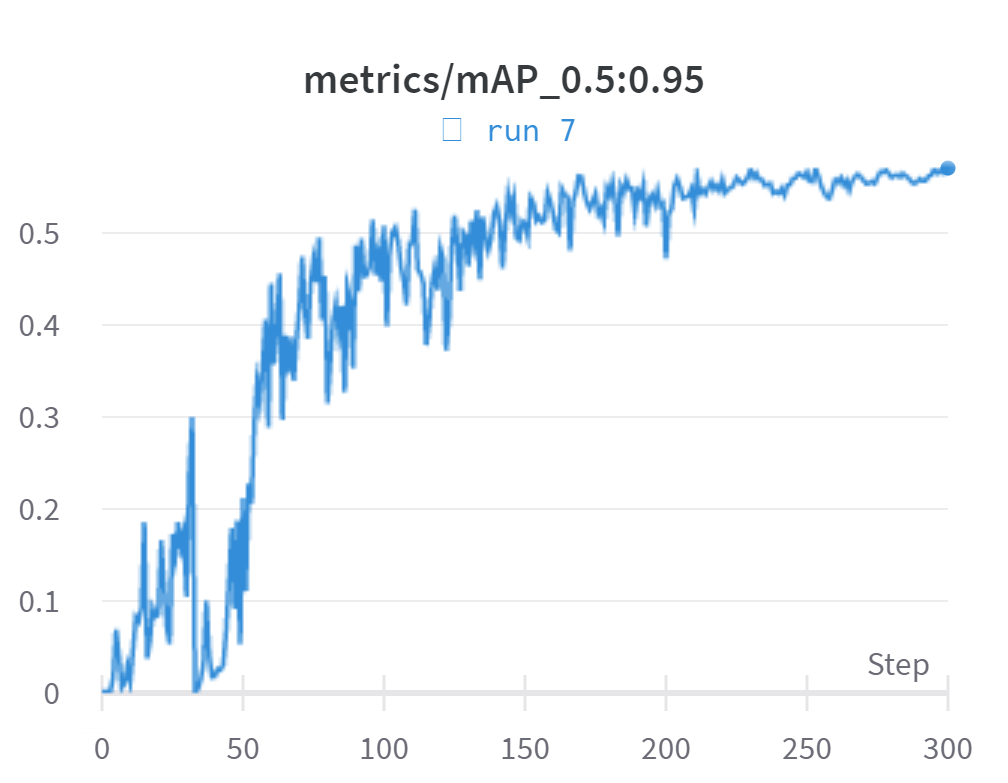
\includegraphics[width=3in]{images/05Testing/run07/Section-1-Panel-0-l24a15v4n}}
\subfloat{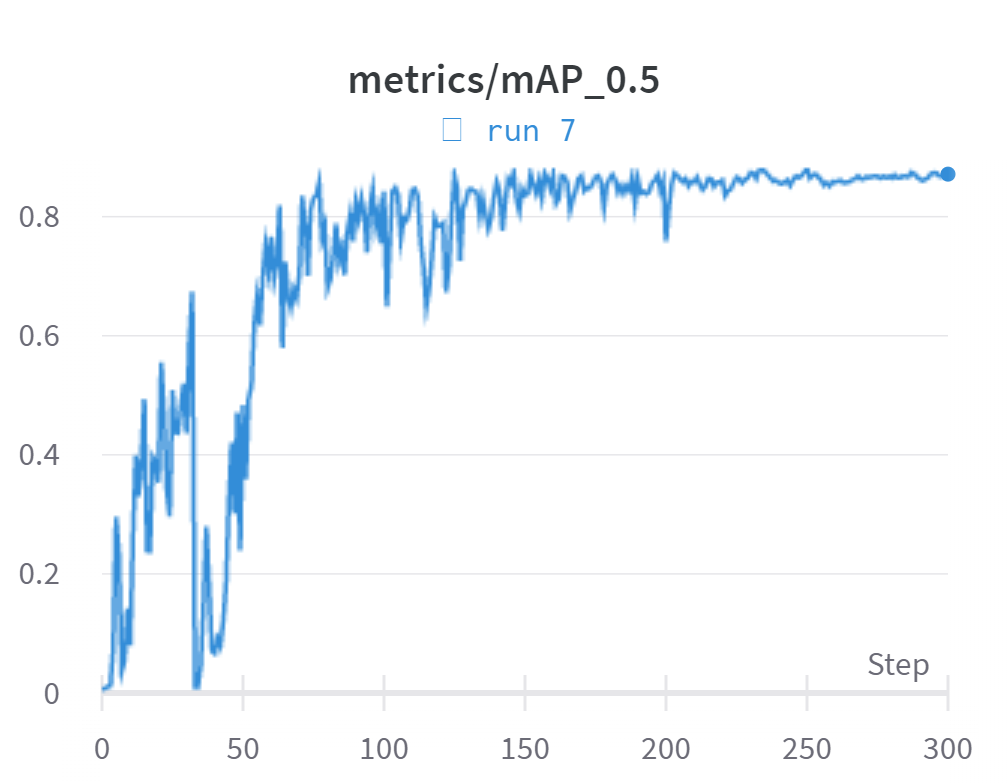
\includegraphics[width=3in]{images/05Testing/run07/Section-1-Panel-1-xq6pmkk16}}\\
\subfloat{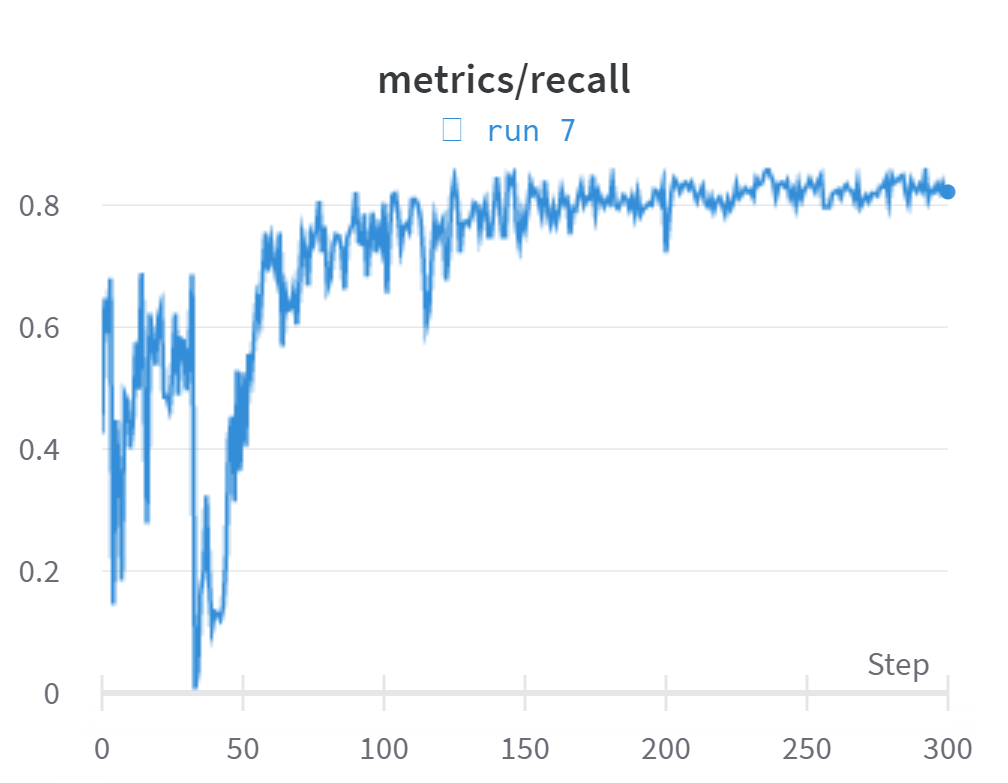
\includegraphics[width=3in]{images/05Testing/run07/Section-1-Panel-2-45rd7tgay}}
\subfloat{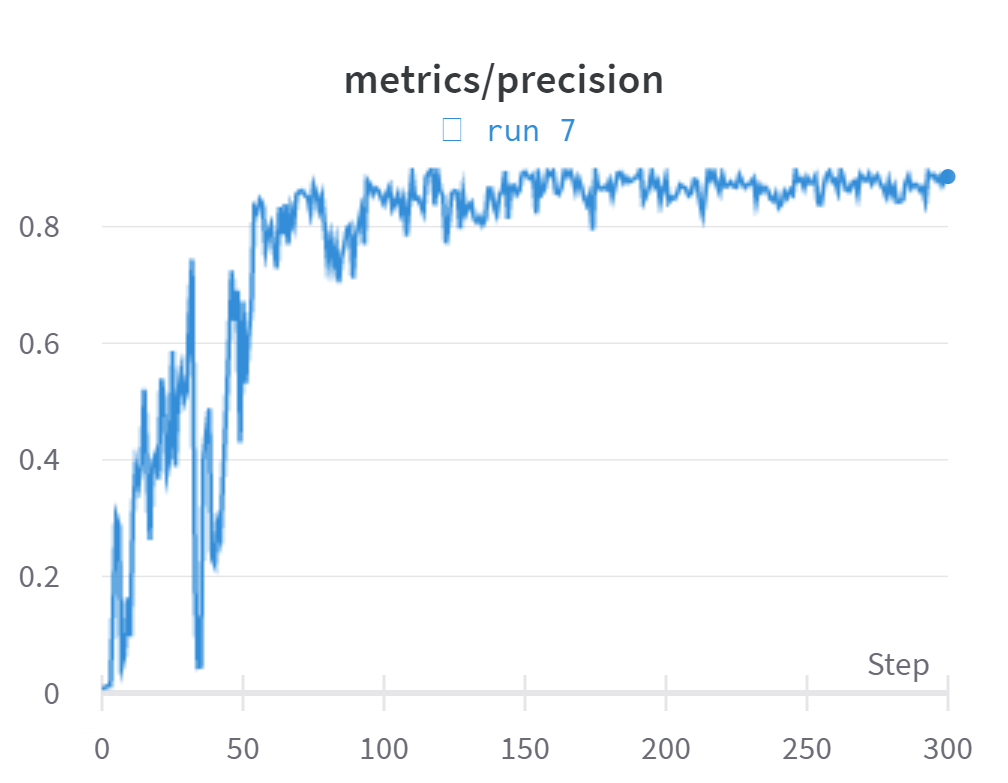
\includegraphics[width=3in]{images/05Testing/run07/Section-1-Panel-3-jsgjesr4f}}\\
\subfloat{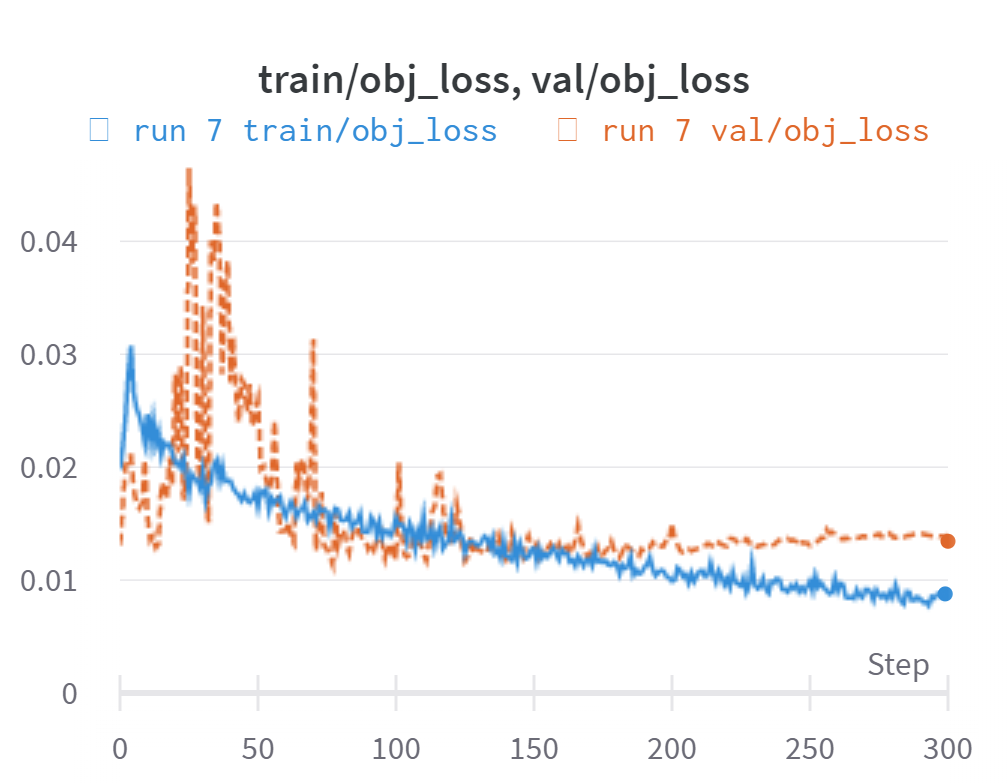
\includegraphics[width=3in]{images/05Testing/run07/Section-1-Panel-4-jgehu72sd}}
\subfloat{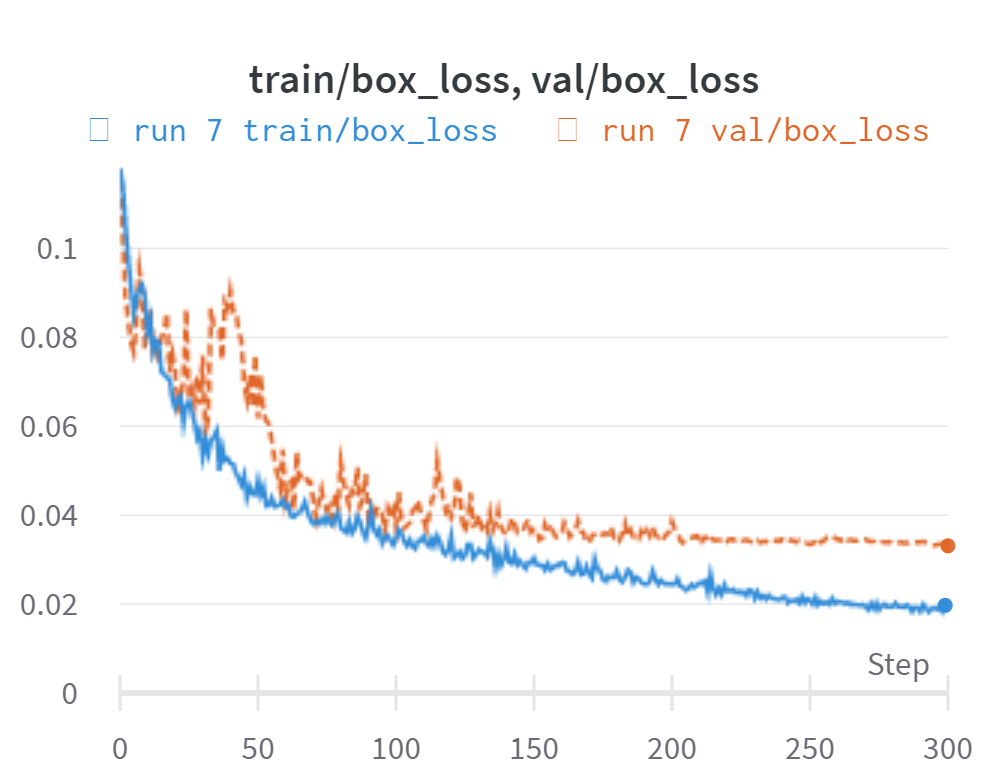
\includegraphics[width=3in]{images/05Testing/run07/Section-1-Panel-5-m94dwffr9}}
\caption{Metrics for Model 7}
\end{figure}

\begin{table}[h!]
\centering
\begin{tabular}{||c c c c c||} 
\hline
Image &  Ground Truth &  Model Count &  Num. Error &    \% Error \\
\hline\hline
37 &            81 &           95 &          14 &  17.283951 \\
39 &            58 &           46 &          12 &  20.689655 \\
41 &            86 &           95 &           9 &  10.465116 \\
44 &           102 &          127 &          25 &  24.509804 \\
\hline
\end{tabular}
\caption{Counts \& errors for Model 7}
\label{count_7}
\end{table}

\section{Source Code}
Source code is hosted on GitHub and can be accessed at \url{https://github.com/adamindeen/CM4105-Honours}.

\section{Project Log}
The project log can be found in the project's Git repository under the filename \verb`log.md`.\\

\paragraph{23/09/2021}
1-hour meeting. Discussed the current method under investigation:\\
1. take input image, turn it into patches
2. use trained GAN to do style transfer on the patches
3. Process ground truth to get the cell markings \verb`validation_steps`
4. reassemble the patches and count the cells.

Received reading pointers:\\
   - GANs and Neural Style Transfer (as a specific application, transformation of horses into zebras with CGANs)
   - ImageJ
   - Yolo

Submitted template matching as a possible alternative solution.

\paragraph{30/09/2021}
No meeting. Continued with reading.

\paragraph{07/10/2021}
Meeting to clarify the project proposal. Project options discussed:\\
- Implement a GAN (such as pix2pix) for style transfer of micrographs into computer-interpretable 'binary' images
- Implement a model to count 'cells' in 'binary' images
- Implement a web interface for an existing model\\

It was clarified that the existing solution is still under development and there is still significant scope for refinement.

\paragraph{08/10/2021}
Completed & submitted Project Proposal & Ethics Form. Project is to implement a machine learning model for cell counting, not a web interface for such a model.\\

Feedback on Project Proposal:\\
- Citations: the link is fine in the proposal but make sure you cite properly in the actual project document. Use Harvard if you can, but if you're using LaTeX, Vancouver might be easier (it's hard to find a decent Harvard LaTeX bib style)
- You're missing the term "semantic segmentation". That's what the "binary" file is - grey for background, black for trichome, white for cell-centre. Semantic segmentation provides a mask showing the "meaning" of each pixel (i.e. which object it belongs to).
- You're missing "evaluation of my technique" in your milestones list. I know it'll probably be an iterative approach (develop method, how good is it? Make it better. How good is it now?), but you can mention evaluation of your own model as one of your objectives. AND you can then say that evaluating such a model is a key technique (how do you know your model is any good?).
- If you wanted to expand your project plan, you might take a "months and milestones" approach, and you start doing that by looking at your deadlines for the honours project. This will be more important later when you might have to pull yourself out of a research rabbit-hole to make sure you complete the project on time (even if it's not "complete" to the standard you want!).\\

Clarification on ethics: the dataset of micrographs is internal to the University and does not create any data protection concerns.

\paragraph{14/10/2021}
1-hour meeting post-Project Proposal submission. Discussed:\\
- Labelme
- Grabcut to process rough binary map produced by high pass filter
- Object detection & region proposal in YOLOv5\\

A possible specification of a project within the bounds of the proposal was suggested: retraining YOLOv5 to detect, localise, and count cyanobacteria cells.

\paragraph{27/10/2021}
Feedback received for Project Proposal:\\

The project proposal is very thorough and clear. There are a couple of places where I think you could improve. You mention research participants, but that doesn’t necessarily fit in with the rest of the proposal (any more), and you’ve named some key techniques but you could do with slightly more detail on some of them. For example, machine learning can be implemented in many ways, and python libraries like keras or pytorch facilitate this. Your project plan is detailed enough that it will see you complete the project in a timely manner, and the background and motivation sections are excellent. Your writing style is lucid and appropriate for the task.

\paragraph{04/11/2021}
No meeting. Continued with reading.

\paragraph{12/11/2021}
Decided to postpone meeting in favour of continuing with Literature Review.

\paragraph{15/11/2021}
In-person meeting discussing the literature review:\\
- Follow a 'here's how it was done, here's why it was good, here's how it relates to my  project' approach
- The example literature reviews represent exactly what is required
- Include abstract & table of contents
- Include *applied* references, i.e. those which can be 'tied back' to the project requirements. For example, YOLO has implementations in both Keras and Pytorch. This is a piece of info worth tying back to the project's non-functional requirements. Another could be a comparison of regularisation functions Adam and SGD

\paragraph{18/01/2022}
30-minute in-person meeting. Revisited the project scope (retrain YOLO on Micropics, repeat if possible) and the state of the project so far (no news).

\paragraph{24/01/2022}
Began familiarisation with YOLO & micropics repo.

\paragraph{25/01/2022}
Began critical appraisal of image annotation tools (Labelstudio vs Labelme).\\
Meeting discussed:
- The process of patching images (if blank patches are to be removed, a new approach will need to be developed since the existing one presumes a processed image with a black background)
- The structure of the final report (Design, Implementation, Evaluation)

\paragraph{01/02/2022}
Meeting
What metrics does YOLO output after training? Keep in mind that an IOU of 20\% is good\\

Report
Structure should include ‘Design’ and ‘Results’ sections
Including a GitHub link might influence professionalism grade
Add more requirements or refine existing ones (the 
Evaluate yolo & other tools
Demonstrate whether it’s a good idea to 
Include paragraph on density estimation, explain why it is likely to be unsuitable (highly varying density of cells across image). Justify YOLO
Have you built the code correctly? Have you built the correct code?\\

Have you tested the hypothesis that giving it more data yields better results
Write a script that removes suffixes from images output by Label Studio
What was a 
Ethics - cover them all
Assume reader will only read the opening and closing\\

Match opening \& closing paragraphs of section
FRACTAL
Write like JSON
Describe graphs
Shamal isn’t a deep learning guy\\

Use the page limit even if you’re repeating yourself
Good comeback for ‘I would like to see more on this\\

If I just read the section titles/ start \& end of each section I should get it
State the obvious\\

3-5 references for poster
No page sums in refs\\

Main meat of the demo is showing the code/explaining the results


\paragraph{23/02/2022}
In-person meeting. Discussed:
- HOG descriptors
- Transfer learning as the basis for retraining YOLO
  - Justify the model used as a basis
- Reducing oscillation (reduce learning rate by factor of 10 or 100)
- The possibility of data processing introducing bias
- Distortion/occlusion/foreshortening of images
- Writing up
  - Write in the order things are done
  - Methodology, Results, and Evaluation are graded separately
  - Read the grading grid
  - Reflection - justify the method used
  - The first and last paragraph of a section, apart from the rest, should make sense
  - If it doesn't correspond to an Aim/Objective, it doesn't count
  - Refer to As\&Os in Conclusion
  
\paragraph{26/02/2022}
Set up DGX \& became familiarised with the system.

\paragraph{15/03/2022}
15-minute Teams meeting. Further discussed DGX setup.

\paragraph{22/03/2022}
Brief in-person discussion:

- Development can continue for the project duration and concurrently with the writeup

\paragraph{24/03/2022}
Email check-in:

- '...Record absolutely everything (screenshots, accuracy etc. etc.). If the conclusion of your project is just “We need to label way more than just 20 images to get good results because the accuracy is pretty terrible with just a few labelled images”, then that is probably a valid conclusion, but make sure you are recording the data as you go so you don’t “lose” any experiments in the write up. Write up absolutely everything you have, whether it works or not.'
- '...I’m planning on taking leave 4-8 April inclusive, but if you desperately need me, I will be checking email infrequently.'

\paragraph{13/04/2022}
Entire 20-image dataset labelled (first pass).

\paragraph{14/04/2022}
Unsuccessfully attempted to set up a DGX Jupyter notebook to run inference.

\paragraph{15/04/2022}
1-hour meeting. Mainly tried to resolve the aforementioned DGX issue without success (another user appears to be occupying all the GPUs). It was decided Google Colab should be used instead while the issue is investigated.

\paragraph{16/04/2022}
Began structuring report according to RGU LaTeX template. Purchased Colab Pro subscription for GPU training.

\paragraph{17/04/2022}
Test run using GPU runtime. Good results.

\paragraph{18/04/2022}
Labelled dataset (2nd run), including partially visible and out-of-focus cells, followed by 2nd run of training. Moved one image each from the validation and test sets to the training set for a 70/30 train/test split, followed by 3rd run of training.

\paragraph{19/04/2022}
4th run of training (increased epochs to 50), with improved results (based on metrics). Updated Jupyter notebook to include script to sum counts for all patches (for each image in the test set).

\paragraph{20/04/2022}
Created spreadsheet to capture model counts vs ground truth counts and determine error (absolute & percentage). Discovered discrepancy between counting performance & metrics (model counts are 2-3x ground truth). 30-minute remote meeting on poster deliverable and report:

- Increasing the training data increased performance (so more labelled data would be good)
- Increasing the labels increased performance (but also increased false positives?)
- Increasing the training time (number of steps?) improved performance (in terms of mAP and count?)
- The problem might not be in missed detection, but rather in false positives
- Does better mAP correlate with better cell count?
- An alternative analysis might calculate error for each patch and then average across the image
- Emphasise the fact that since a base YOLO model would be unsuitable, it was retrained 4 times, showing a development process
- The dataset is not perfect - only 1 expert annotator
- Mention the selection of YOLOv5 model in Design - speed? Portability?

Submitted. 

\paragraph{21/04/2022}
Continued with writeup. Added Requirements Specification and section on labelling tools to Methodology

\paragraph{22/04/2022}
Development:
- General cleanup of Colab notebook
- Added evaluation section with DataFrame
- Trained model based on YOLOv5l

Report:
- Made progress in Design
- Started Implementation

\paragraph{23/04/2022}
Contacted school office to arrange degree show session. 

Report:
- Made substantial progress in Design \& Implementation chapters
- Added project proposal \& ethics form to appendix

\paragraph{24/04/2022}
Report:
- Made some progress in Design

\paragraph{25/04/2022}
Trained models 6 \& 7 based on YOLOv5l, with excellent results.

Report:
- Added poster to appendix
- Made substantial progress in Testing

\paragraph{26/04/2022}
Submitted incomplete draft of the final report for feedback. Discussed the report deliverable as a whole in the final meeting (fractal writing, reference to figures within the text, proofreading)

\paragraph{27/04/2022}
Degree show. Presentation to supervisor & second marker was mostly successful with some lessons learned (future work must be clarified)

\paragraph{28/04/2022}
Feedback received for initial draft. All implemented.

\paragraph{29/05 - 06/05/2022}
Continued work on final report.

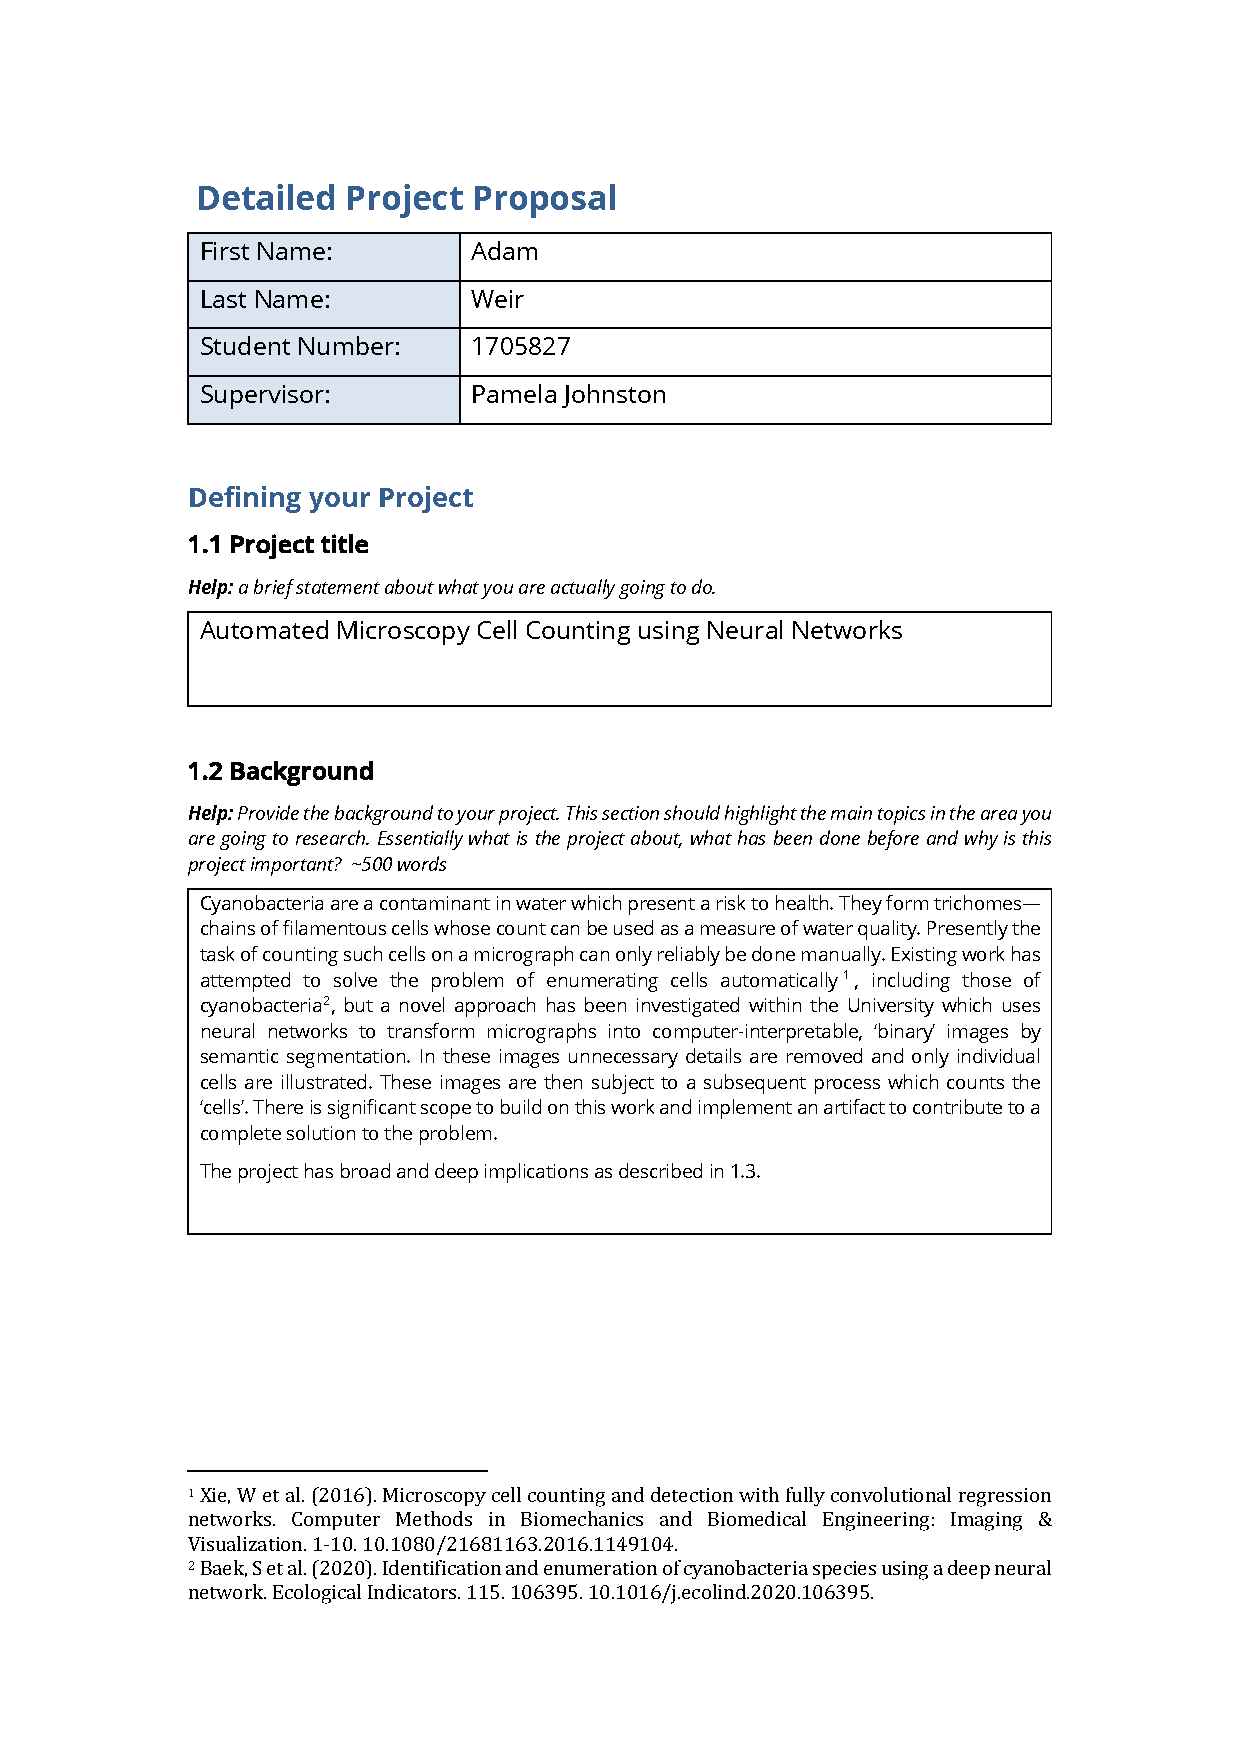
\includepdf[scale=0.9, pages=1, pagecommand=\section{Project Proposal}]{docs/proposal.pdf}
\includepdf[scale=0.9, pages=2-]{docs/proposal.pdf}

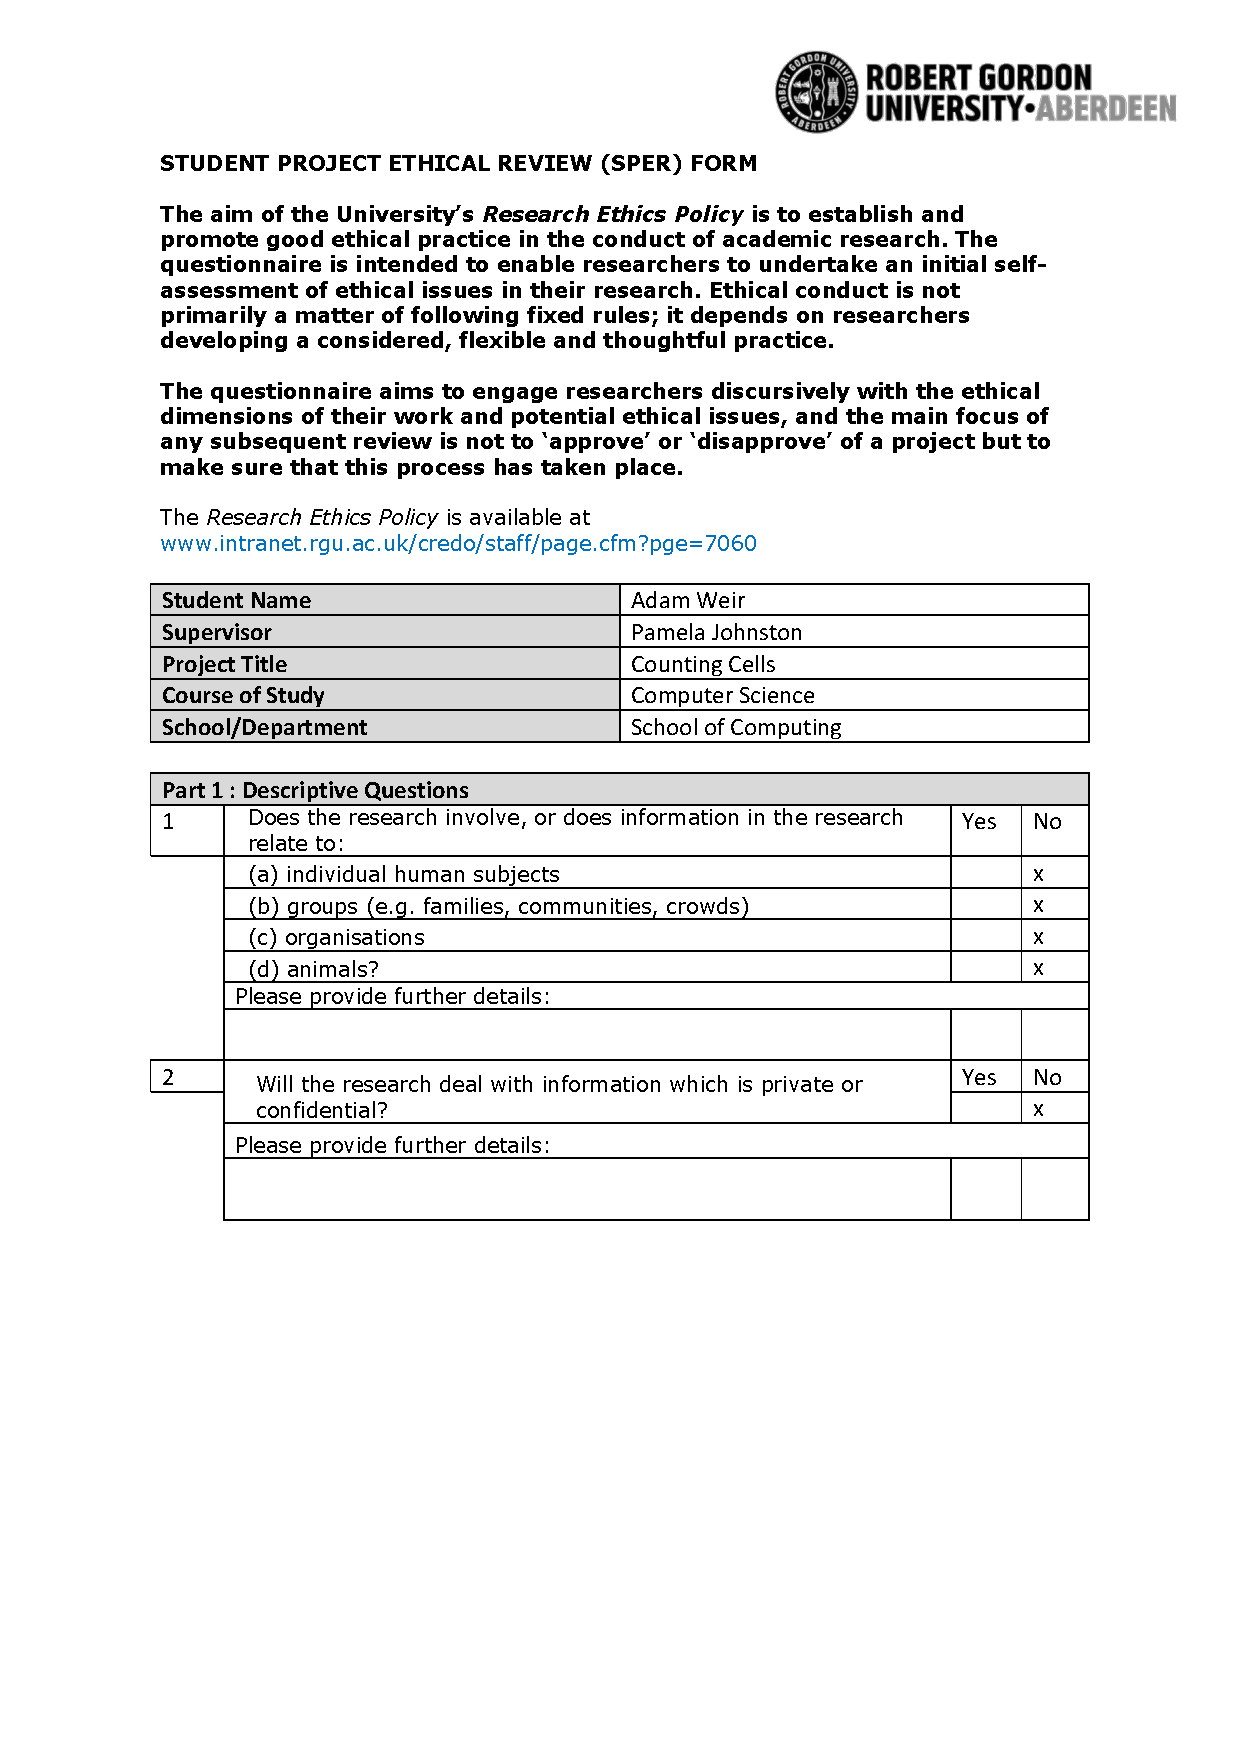
\includepdf[scale=0.9, pages=1, pagecommand=\section{Ethics Form}]{docs/ethics.pdf}
\includepdf[scale=0.9, pages=2-]{docs/ethics.pdf}

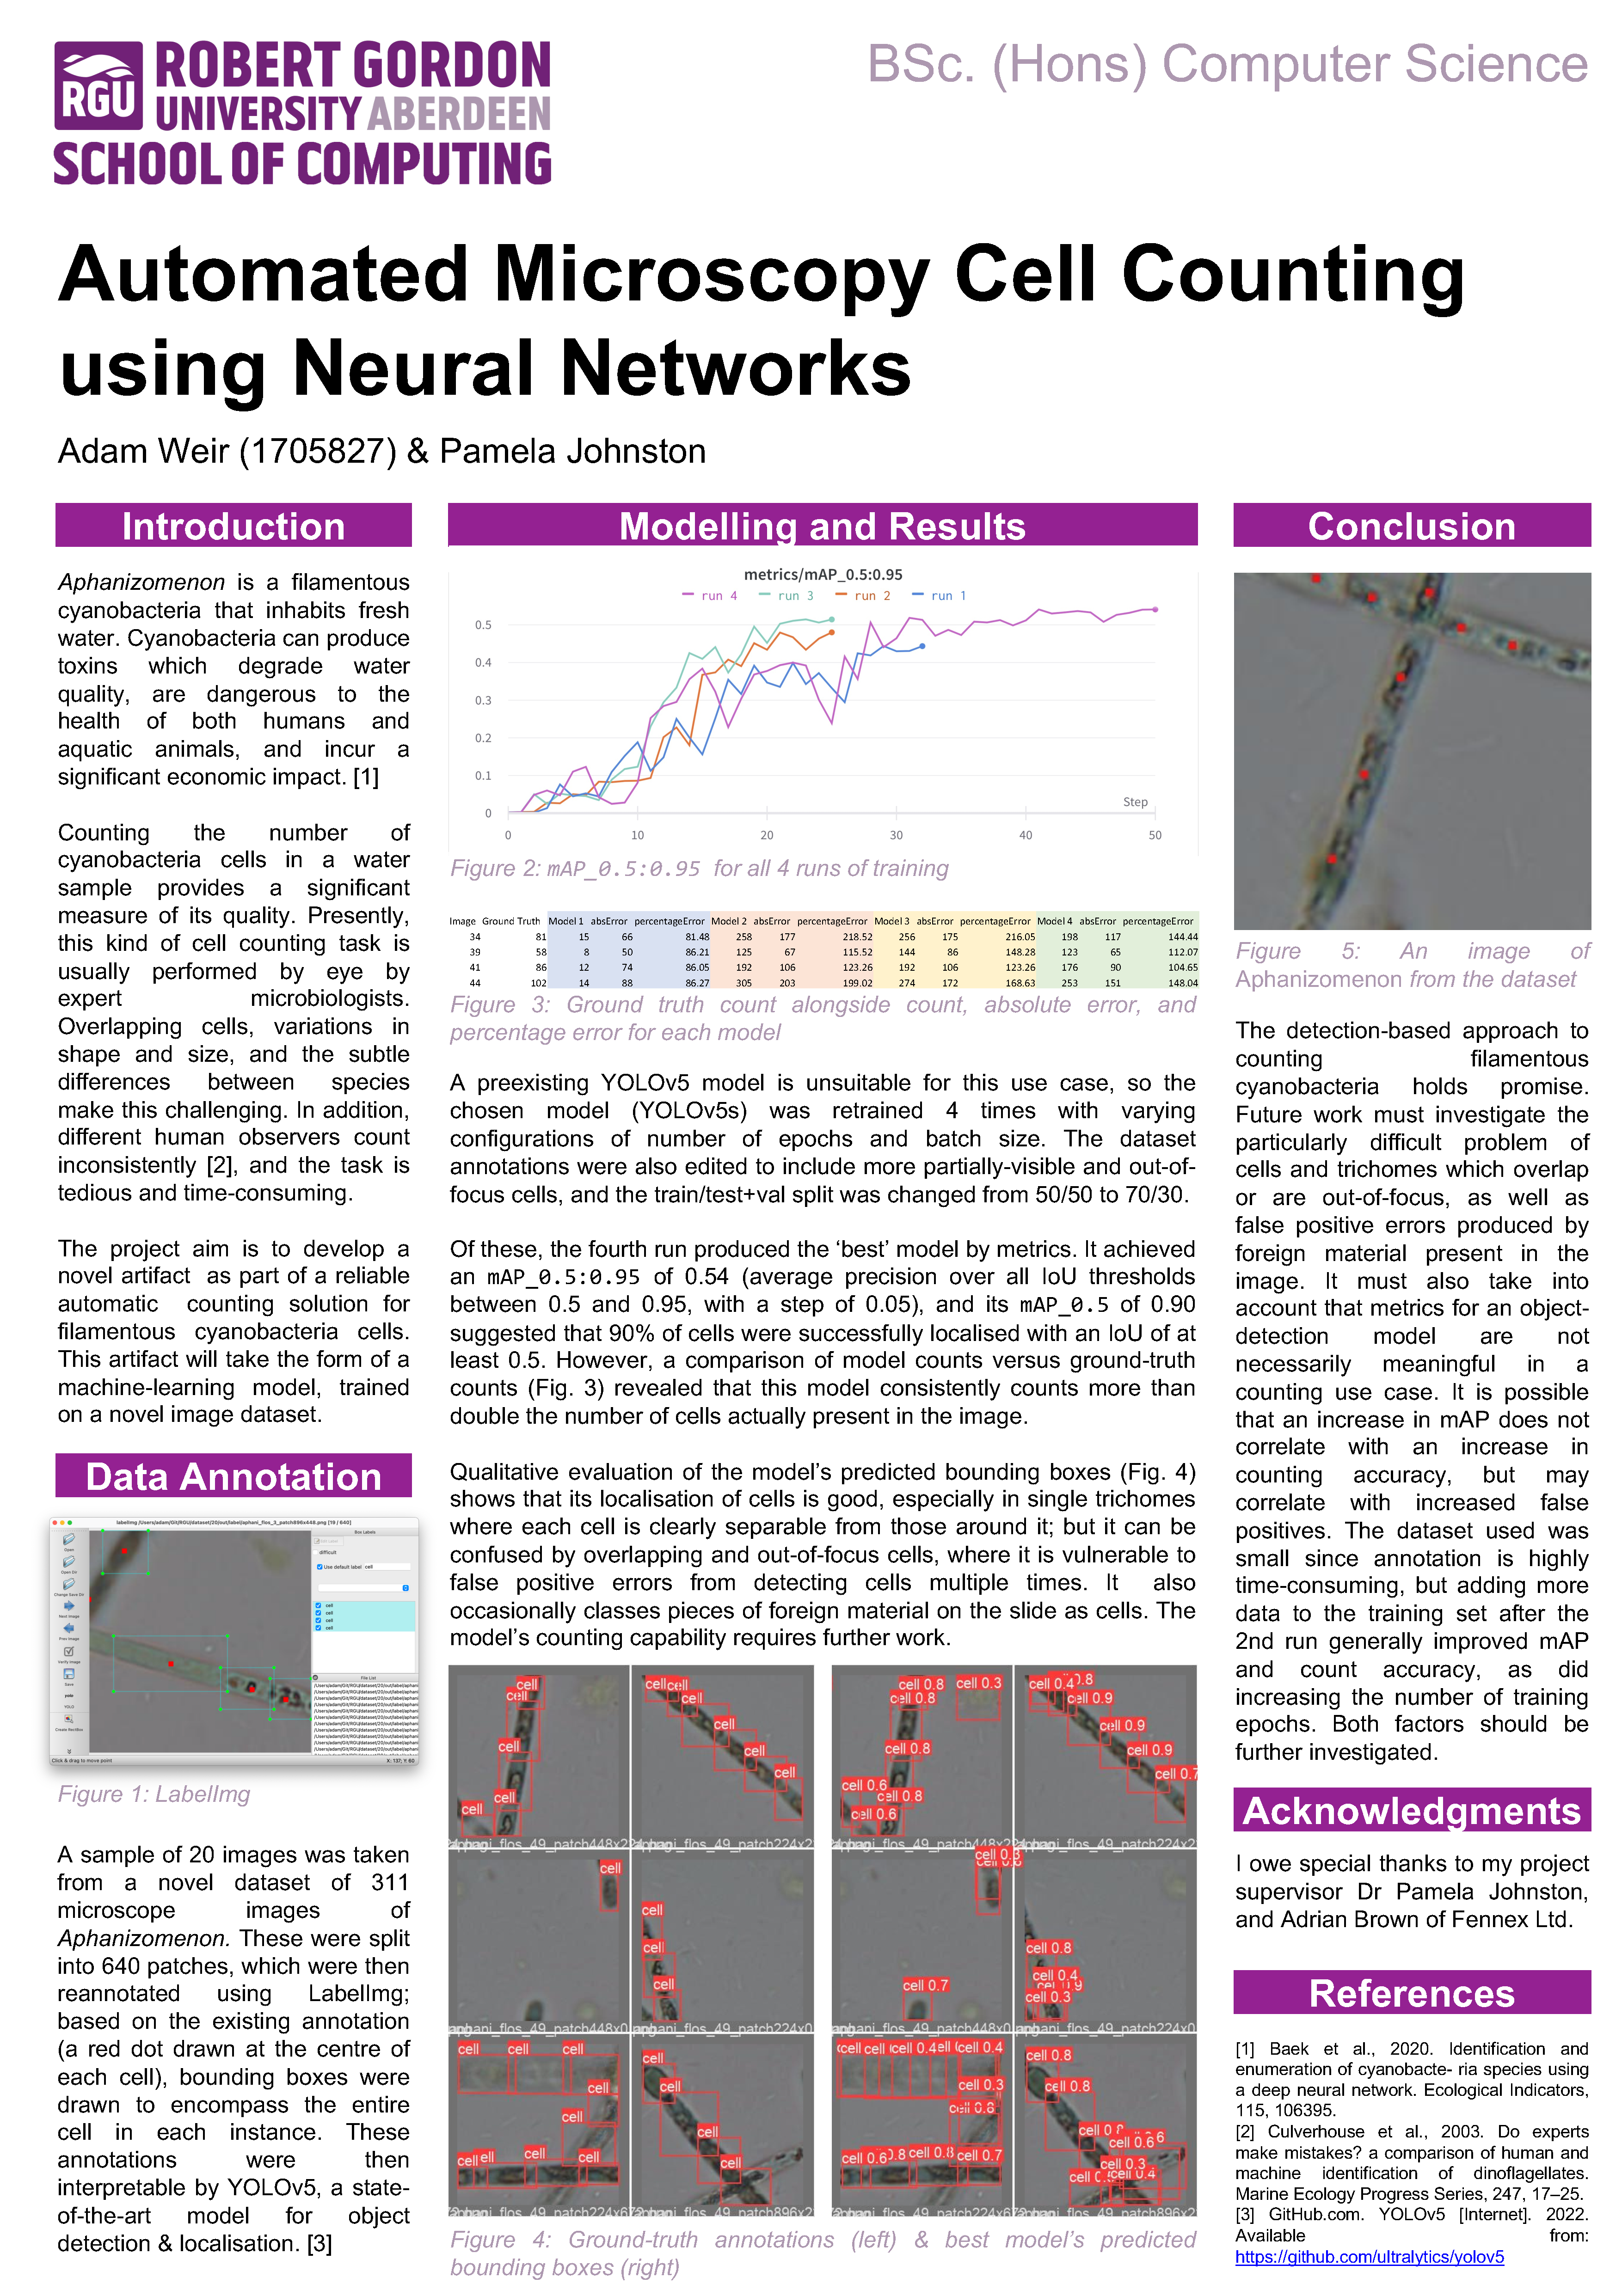
\includepdf[scale=0.8, pages=1, pagecommand=\section{Degree Show Poster}]{docs/poster.pdf}

\end{appendices}